%% BioMed_Central_Tex_Template_v1.06
%%                                      %
%  bmc_article.tex            ver: 1.06 %
%                                       %

%%IMPORTANT: do not delete the first line of this template
%%It must be present to enable the BMC Submission system to
%%recognise this template!!

%%%%%%%%%%%%%%%%%%%%%%%%%%%%%%%%%%%%%%%%%
%%                                     %%
%%  LaTeX template for BioMed Central  %%
%%     journal article submissions     %%
%%                                     %%
%%          <8 June 2012>              %%
%%                                     %%
%%                                     %%
%%%%%%%%%%%%%%%%%%%%%%%%%%%%%%%%%%%%%%%%%


%%%%%%%%%%%%%%%%%%%%%%%%%%%%%%%%%%%%%%%%%%%%%%%%%%%%%%%%%%%%%%%%%%%%%
%%                                                                 %%
%% For instructions on how to fill out this Tex template           %%
%% document please refer to Readme.html and the instructions for   %%
%% authors page on the biomed central website                      %%
%% http://www.biomedcentral.com/info/authors/                      %%
%%                                                                 %%
%% Please do not use \input{...} to include other tex files.       %%
%% Submit your LaTeX manuscript as one .tex document.              %%
%%                                                                 %%
%% All additional figures and files should be attached             %%
%% separately and not embedded in the \TeX\ document itself.       %%
%%                                                                 %%
%% BioMed Central currently use the MikTex distribution of         %%
%% TeX for Windows) of TeX and LaTeX.  This is available from      %%
%% http://www.miktex.org                                           %%
%%                                                                 %%
%%%%%%%%%%%%%%%%%%%%%%%%%%%%%%%%%%%%%%%%%%%%%%%%%%%%%%%%%%%%%%%%%%%%%

%%% additional documentclass options:
%  [doublespacing]
%  [linenumbers]   - put the line numbers on margins

%%% loading packages, author definitions

%\documentclass[twocolumn]{bmcart}% uncomment this for twocolumn layout and comment line below
\documentclass{bmcart}

%%% Load packages
\usepackage{amsthm,amsmath}
\usepackage{natbib}
%\RequirePackage[authoryear]{natbib}% uncomment this for author-year bibliography
\usepackage{hyperref}
\usepackage[utf8]{inputenc} %unicode support
%\usepackage[applemac]{inputenc} %applemac support if unicode package fails
%\usepackage[latin1]{inputenc} %UNIX support if unicode package fails

\usepackage{graphicx}
\usepackage{epstopdf}
\usepackage{todonotes}
%\usepackage{amsmath}
\usepackage{threeparttable}
%%\usepackage{bibentry}
\usepackage{float}
%\usepackage{booktabs}


%%%%%%%%%%%%%%%%%%%%%%%%%%%%%%%%%%%%%%%%%%%%%%%%%
%%                                             %%
%%  If you wish to display your graphics for   %%
%%  your own use using includegraphic or       %%
%%  includegraphics, then comment out the      %%
%%  following two lines of code.               %%
%%  NB: These line *must* be included when     %%
%%  submitting to BMC.                         %%
%%  All figure files must be submitted as      %%
%%  separate graphics through the BMC          %%
%%  submission process, not included in the    %%
%%  submitted article.                         %%
%%                                             %%
%%%%%%%%%%%%%%%%%%%%%%%%%%%%%%%%%%%%%%%%%%%%%%%%%


\def\includegraphic{}
\def\includegraphics{}



%%% Put your definitions there:
%\startlocaldefs
%\endlocaldefs


%%% Begin ...
\begin{document}

%%% Start of article front matter
\begin{frontmatter}

\begin{fmbox}
\dochead{Research}

%%%%%%%%%%%%%%%%%%%%%%%%%%%%%%%%%%%%%%%%%%%%%%
%%                                          %%
%% Enter the title of your article here     %%
%%                                          %%
%%%%%%%%%%%%%%%%%%%%%%%%%%%%%%%%%%%%%%%%%%%%%%

\title{Re-interpreting biomedical database content as ontologies for enhanced querying}

%%%%%%%%%%%%%%%%%%%%%%%%%%%%%%%%%%%%%%%%%%%%%%
%%                                          %%
%% Enter the authors here                   %%
%%                                          %%
%% Specify information, if available,       %%
%% in the form:                             %%
%%   <key>={<id1>,<id2>}                    %%
%%   <key>=                                 %%
%% Comment or delete the keys which are     %%
%% not used. Repeat \author command as much %%
%% as required.                             %%
%%                                          %%
%%%%%%%%%%%%%%%%%%%%%%%%%%%%%%%%%%%%%%%%%%%%%%

\author[
   addressref={aff1},                   % id's of addresses, e.g. {aff1,aff2}
   corref={aff1},                       % id of corresponding address, if any
   noteref={n1},                        % id's of article notes, if any
   email={fss3@cin.ufpe.br}   % email address
]{\inits{FSS}\fnm{Filipe} \snm{Santana da Silva}}

\author[
addressref={aff2},                   % id's of addresses, e.g. {aff1,aff2}
%corref={aff2},                       % id of corresponding address, if any
noteref={n1},                        % id's of article notes, if any
email={robert.hoehndorf@kaust.edu.sa}   % email address
]{\inits{RH}\fnm{Robert} \snm{Hoehndorf}}

\author[
addressref={aff1},                   % id's of addresses, e.g. {aff1,aff2}
%corref={aff1},                       % id of corresponding address, if any
noteref={n1},                        % id's of article notes, if any
%email={fred@cin.ufpe.br}   % email address
]{\inits{FF}\fnm{Fred} \snm{Freitas}}

\author[
addressref={aff3},                   % id's of addresses, e.g. {aff1,aff2}
%corref={aff3},                       % id of corresponding address, if any
noteref={n1},                        % id's of article notes, if any
email={stefan.schulz@medunigraz.at}   % email address
]{\inits{SS}\fnm{Stefan} \snm{Schulz}}


%%%%%%%%%%%%%%%%%%%%%%%%%%%%%%%%%%%%%%%%%%%%%%
%%                                          %%
%% Enter the authors' addresses here        %%
%%                                          %%
%% Repeat \address commands as much as      %%
%% required.                                %%
%%                                          %%
%%%%%%%%%%%%%%%%%%%%%%%%%%%%%%%%%%%%%%%%%%%%%%

\address[id=aff1]{%                           % unique id
  \orgname{Centro de Inform\'{a}tica, Universidade Federal de Pernambuco}, % university, etc
  \street{Av. Jornalista Anibal Fernandes},                     %
  \postcode{50.740-560}                                % post or zip code
  \city{Recife},                              % city
  \cny{Brazil}                                    % country
}

\address[id=aff2]{%
  \orgname{Computational Bioscience Research Center, King Abdullah University of Science and Technology},
%  \street{Thuwal, 6900},
  \postcode{23955-6900}
  \city{Thuwal},
  \cny{Kingdom of Saudi Arabia}
}

\address[id=aff3]{%
	\orgname{Institut f\"{u}r Medizinische Informatik, Statistik und Dokumentation, Medzinische Universit\"{a}t Graz},
	\street{Auenbruggerplatz 2},
	\postcode{8036}
	\city{Graz},
	\cny{Austria}
}

%%%%%%%%%%%%%%%%%%%%%%%%%%%%%%%%%%%%%%%%%%%%%%
%%                                          %%
%% Enter short notes here                   %%
%%                                          %%
%% Short notes will be after addresses      %%
%% on first page.                           %%
%%                                          %%
%%%%%%%%%%%%%%%%%%%%%%%%%%%%%%%%%%%%%%%%%%%%%%

\begin{artnotes}
%\note{Sample of title note}     % note to the article
\note[id=n1]{Equal contributor} % note, connected to author
\end{artnotes}

\end{fmbox}% comment this for two column layout

%%%%%%%%%%%%%%%%%%%%%%%%%%%%%%%%%%%%%%%%%%%%%%
%%                                          %%
%% The Abstract begins here                 %%
%%                                          %%
%% Please refer to the Instructions for     %%
%% authors on http://www.biomedcentral.com  %%
%% and include the section headings         %%
%% accordingly for your article type.       %%
%%                                          %%
%%%%%%%%%%%%%%%%%%%%%%%%%%%%%%%%%%%%%%%%%%%%%%

\begin{abstractbox}

\begin{abstract} % abstract
%\parttitle{} %if any
\textbf{Motivation:} 
Although content from biomedical domain ontologies constitutes a major source for biological databases, current querying strategies mainly follow the syntax of the underlying database scheme and use ontologies mainly as domain vocabularies. 
We address this shortcoming by ontology grounding, an approach that makes hidden ontological assumptions of databases explicit and exploits the representational richness of the related domain ontologies. The result is an ontological resource, in which database and domain ontology content is seamlessly integrated as a large set of OWL axioms, underpinned by formal-ontological principles. 
This resource is generated fully automatically, guided by a set of manually crafted, database-specific design patterns.  \\
\textbf{Results:} We applied ontology grounding to a database extract (Uniprot, Ensembl) on amino acid metabolism. Ontology completeness and correctness were tested using pre-formulated competence questions as description logics (DL) queries, encompassing proteins, biological processes, molecular activities and dysfunctional phenotypes. The expected results could be reproduced by the description logics reasoner. Benchmark tests showed moderate scalability. Real-world use of this method still depends on large-scale content filtering and modularization prior to ontology creation.

\textbf{Availability:} \href{http://www.cin.ufpe.br/\textasciitilde integrativo}{http://www.cin.ufpe.br/\textasciitilde integrativo}

%\parttitle{Second part title} %if any
%Text for this section.
\end{abstract}

%%%%%%%%%%%%%%%%%%%%%%%%%%%%%%%%%%%%%%%%%%%%%%
%%                                          %%
%% The keywords begin here                  %%
%%                                          %%
%% Put each keyword in separate \kwd{}.     %%
%%                                          %%
%%%%%%%%%%%%%%%%%%%%%%%%%%%%%%%%%%%%%%%%%%%%%%

\begin{keyword}
\kwd{sample}
\kwd{article}
\kwd{author}
\end{keyword}

% MSC classifications codes, if any
%\begin{keyword}[class=AMS]
%\kwd[Primary ]{}
%\kwd{}
%\kwd[; secondary ]{}
%\end{keyword}

\end{abstractbox}
%
%\end{fmbox}% uncomment this for twcolumn layout

\end{frontmatter}

%%%%%%%%%%%%%%%%%%%%%%%%%%%%%%%%%%%%%%%%%%%%%%
%%                                          %%
%% The Main Body begins here                %%
%%                                          %%
%% Please refer to the instructions for     %%
%% authors on:                              %%
%% http://www.biomedcentral.com/info/authors%%
%% and include the section headings         %%
%% accordingly for your article type.       %%
%%                                          %%
%% See the Results and Discussion section   %%
%% for details on how to create sub-sections%%
%%                                          %%
%% use \cite{...} to cite references        %%
%%  \cite{koon} and                         %%
%%  \cite{oreg,khar,zvai,xjon,schn,pond}    %%
%%  \nocite{smith,marg,hunn,advi,koha,mouse}%%
%%                                          %%
%%%%%%%%%%%%%%%%%%%%%%%%%%%%%%%%%%%%%%%%%%%%%%

%%%%%%%%%%%%%%%%%%%%%%%%% start of article main body
% <put your article body there>

%%%%%%%%%%%%%%%%
%% Background %%
%%
\section*{Introduction}
Biomedical research increasingly depends on large databases, such as UniProt  \citep{UniProtConsortium2014} or Ensembl \citep{Cunningham2014}. The formulation of database queries and the correct interpretation of query results requires knowledge of the database structure as well as implicit background knowledge about the way data is produced and recorded. 
Such background knowledge may vary between users, thus biasing uniform data interpretation. 

There have been several attempts to enhance data retrieval by formal ontologies like ontology-based data access (OBDA) \citep{Poggi2008} or the combination of ontologies with machine learning \citep{Lehmann2009}. However, such approaches require in-depth manual interpretation of the finally retrieved content; and the representation of data entities  as individuals (ABox elements in description logics) results in high processing cost \citep{Hustadt2005}.

Accordingly, the current situation regarding the (semi-)automated support for database content retrieval and interpretation is characterized by a concurrent and continuous evolution of high-quality structured knowledge resources, whereas less progress can be seen regarding their interoperability and ontological underpinning. Superficial use of ontologies - just as vocabularies - restricts their applicability. We hypothesise that with a formally explicit view on biomedical data as provided by principled ontologies, users are better served to integrate, retrieve, validate and interpret these data, due to automated classification and consistency checking provided by Description Logics (DL) representation and reasoning \citep{Baader2007g}. 
% classifiers, like Fact++ \citep{Tsarkov2006}.

We investigate this hypothesis by proposing a model for the seamless integration of the content of biological databases and ontologies, guided by formal-ontological principles \citep{Smith2007}, which enforce univocal interpretation of database content in order to improve (semi-)automated data interpretation and understanding. Ontology-level content in identified in databases, and axiomatized under an upper level ontology. Thus it delivers a homogeneous representation of data, linked to (modules of) existing ontologies.
The proposed approach might be applied to enhance database curation, as new statements extracted from publications and recorded in databases can be tested for adequacy. Supported by description logics (DL) based reasoning, it might enable validation using DL Query as an expressive and simple query language based on DL syntax and semantics. 

We will substantiate this claim by investigating a subset of biomedical ontologies and databases. We (i) propose an ontology-based framework that makes explicit both database content and the domain entities denoted thereby; (ii) relate this framework to current workflows in which life science data and knowledge are acquired and processed; (iii) implement an example ontology from real data as an exemplar for database-ontology integration; (iv) validate it by demonstrating how querying is done by using DL Query; and (vi) experimentally assess correctness and scalability.

The biological use case is addressed by Competency Questions (CQs) \citep{Gruninger1994} as DL queries on the metabolism of small molecules in model organisms, encompassing physiological processes as well as phenotypical changes in dysfunctional  metabolism. The examples make use of UniProt, NCBI Taxonomy \citep{NCBI2015}, Ensembl\citep{Cunningham2014}, SNOMED CT \citep{IHTSDO2015}, GO \citep{Gene2014a}, ChEBI \citep{Hastings2013} and PR \citep{Natale2014}, organized under the upper domain ontology BioTopLite (BTL2) \citep{Schulz2012}. Our approach capitalizes on previous work about the formalization of tabular representations in scientific literature \citep{Santana2011b} and models of structured clinical information \citep{Martinez-Costa2015}.


%Hypotheses and findings are generated in biomedical research based on gathering data from experiments, publications, and databases like UniProt \citep{UniProtConsortium2014} or Ensembl \citep{Cunningham2014}. In the biomedical field, the exploration of this contents is usually performed manually or (partly) supported by retrieval tools, e.g. by STRING \citep{Szklarczyk2014}, or BLAST \citep{Altschup1990}. Some works highlight the need and importance of database interpretation for the biomedical domain \citep{Carnielli2015,Laukens2015}.

%Moreover, the interpretation of these results may be biased by the researchers' capabilities, by the sheer size and heterogeneity of the sources, or by technical limitations \citep{Triplet2011,Laukens2015}. It may result in ambiguous interpretation of data, the non-observance of records that may be crucial for a given problem, or by the user inability to query and filter a dataset, or the elevated processing costs related to massive datasets.
%
%On the other hand, others tools like ontology-based data access (OBDA) \citep{Poggi2008} -related applications enhance data retrieval by ontologies, which serve as a query vocabulary -- e.g. within SPARQL \citep{Harris2013} endpoints. By using, one gains the ability to integrate heterogeneous and massive data sources. Other tools rely on machine learning to interpret databases according to an ontological background \citep{Lehmann2009}. The retrieval of OBDA-based approaches, like SPARQL endpoints, fairly supports reasoning that goes beyond what is available in current relational queries \citep{Angles2008a}. 
%
%However, such approaches are limited by the need of user intervention, e.g. the manual interpretation of the finally retrieved content, and the ontology population with data. Here, the interpretation problem is still present, as well as the raise of processing costs. OBDA and machine learning approaches frequently rely on the representation of data entities as individuals (ABox elements in DL jargon), which results in high processing cost \citep{Hustadt2005}, with or without computer-assisted reasoning.
%
%Accordingly, the current situation regarding the (semi-)automated support for database content retrieval and interpretation is characterized by a concurrent and continuous evolution of high-quality structured knowledge resources, whereas less progress can be seen regarding their usage, interoperability and ontological grounding. Thus, the interpretation of results is frequently left to the users, and influenced by implicit background assumptions that may vary between users. 
%
%Apart from that, the usage of ontologies only to enable data integration and retrieval restricts its applicability and justification. With a formalized view of biomedical data provided by ontologies, we are able to integrate, retrieve, validate and derive assumptions from it, mainly due to automated classification and consistency checking delivered by Description Logics (DL) \citep{Baader2007g} classifiers, like HermiT \citep{Glimm2014}.
%
%We address this shortcoming by advocating a seamless integration of database and ontology content, underpinned by formal-ontological principles \citep{Smith2007}, which enforce an univocal interpretation of the database content. In other words, we emphasize ontological grounding of databases as a mean enable (semi-)automated data interpretation and understanding.
%Ontological grounding means to identify ontology-level content in databases, and to axiomatize it under an upper level ontology. It delivers a homogeneous representation of data, linked to (parts of) existing ontologies. 
%
%Ontological grounding can be applied to enhance database curation, as new statements extracted from recent publications and recorded in databases can be ontologically grounded and tested for adequacy inside the biological domain.  As this process is supported by automated reasoning, it enables a rigorous validation supported by an expressive query language (DL Query). 
%
%A DL Query uses the semantics and reasoning procedures of DL, which allow querying across several databases at the same time, thus decreasing the costs of database integration.  This "ontological grounding" is based on previous work on the formalization of tabular representations in scientific literature \citep{Santana2011b} and models of structured clinical information \citep{Martinez-Costa2015}.
%
%In this sense, we hypothesise and demonstrate that this enables more powerful queries, supported by machine reasoning.  To this end, we will (i) analyse a subset of biomedical ontologies and databases; (ii) propose an ontology-based framework that makes explicit both database content and the domain entities denoted thereby; (iii) relate this solution to current workflows in which life science data and knowledge are acquired and processed; (iv) implement an example ontology from real data as an exemplar for data integration across ontologies and databases; (v) validate this example by demonstrating how querying becomes simpler and more user-friendly; (vi) perform an experiment to assess the scalability of the approach. 
%
%The biological use case is addressed Competency Questions (CQs) \citep{Gruninger1994} as DL queries. They range from how data related to a specific metabolism overlap in biological databases for certain model organisms, to phenotypes from dysfunctional metabolism. Our examples make use of UniProt, NCBI Taxonomy \citep{NCBI2015}, Ensembl, SNOMED CT \citep{Donnelly2006} , GO \citep{Gene2014a}, ChEBI \citep{Hastings2013} and PR \citep{Natale2014}, organized under the upper domain ontology BioTopLite (BTL2) \citep{Schulz2013}. 



\section*{Background}
\subsection{Formal ontologies}

Formal ontologies are centred on classes of individual entities. Together with a set of binary relations and operators in a logic-based language such as a DL dialect, they constitute formal axioms. Axioms are limited to statements about what is universally true for all members of a class or a class-like expression, e.g. that all nucleic acid molecules contain nucleotides, or that all adenine molecules are nucleotides. The construction of (formal) ontologies should obey principled criteria \citep{Spear2006} and good practice guidelines \citep{Schulz2012}. Important principles are (i) naming conventions \citep{Schober2009}; (ii) mutually disjoint upper-level classes like \emph{Process} or \emph{Quality} as a fundamental ordering framework; and, (iii) a limited set of canonical relations \citep{Smith2005}. 

We distinguish \emph{ontology content} properly from both the notions of \emph{knowledge} \citep{Naturwissenschaften2014} and \emph{data}. Knowledge, in a broader sense \citep{Rector2008}, emcompasses assertions about what is frequently associated or what is true by default. This is beyond the scope of formal ontologies. Data, in contrast, are first of all information entities in a database. Like words in a text, data elements constitute denoting entities. 
%Their interpretation is often blurred by use-mention confusion, i.e. mixing data items with the things they denote. 
In databases, the interpretation of data elements is determined by the use cases embedded in the underlying schema. The distinction between what is a data element and what is denoted by it is often neglected and leads to use-mention confusions. Formal ontologies must enforce this distinction: 
all data items are instances of a specific class like \textit{information object} in BTL2, or \textit{generically dependent continuant} in BFO, whereas the things data items denote are manifold: individuals, classes, or even nothing \citep{Schulz2011a}.

%Formal ontologies present mostly extensive (poly-) hierarchies of representational units, named classes, related by a limited set of binary relations. Ontologies are centred around classes. Together with a set of binary relations and logical operators in a logic-based language, e.g., DL, they constitute formal axioms.  Axioms state what is universally true for all members of a class or a class-like expression. For instance, all nucleic acid molecules contain nucleotides, or all adenine molecules are nucleotide molecules.
%
%The construction of (formal) ontologies should obey principled criteria \citep{Spear2006} and good practice guidelines \citep{Schulz2012}. Important principles are (i) naming conventions \citep{Schober2009}; (ii) mutually disjoint upper-level classes like Process or Quality as a fundamental ordering framework; and, (iii) a generally small set of canonical relations \citep{Smith2005}, such as ‘has participant’ or ‘has part’. Both top-level classes and canonical relations are usually supplied by top-level ontologies, such as BFO \citep{Spear2006}, RO \citep{Smith2005}, or BTL2.
%
%We distinguish ontology content properly from both the notions of knowledge (Schulz and Jansen, 2013) and data. Regarding knowledge\footnote{In a broader sense, Cf. \citep{Rector2008}}, assertions about what is frequently associated or only true by default can- not be straightforwardly expressed by formal ontologies. Regarding data, interpretation is often blurred by use-mention confusion, i.e. mixing data items with the things they denote. In databases, the interpretation of data elements is determined by the use cases embedded in the underlying schema. The distinction between what is a data element and what is its referent is often implicit. Formal ontologies should enforce this distinction: data items are instances of information content entities, whereas the things data items denote are manifold: individuals, classes, or even nothing\citep{Schulz2011a}.

\subsection{Interpreting databases with ontologies}
Databases and less-principled domain ontologies leave the real nature of the entities as well as and the circumstances of denotation underspecified, assuming that this is intuitively known by the users and interpreted accordingly within the expected context of use. An example is ``Human", which may denote an individual person, the class \textit{Homo sapiens}, the quality of an object belonging to the taxon \textit{Homo sapiens} \citep{Schulz2008}, or a population of humans. In a similar vein, ``Animal" could be interpreted as including the class \textit{Homo sapiens}, in the context of Biology or excluding it, e.g. in the context of Law. Such ambiguities underline the need to make hidden assumptions explicit, which is the main rationale for the ontological grounding mechanism as described in the following. 
Content retrieval applications that use existing domain ontologies as vocabularies, like the ones derived from OBDA might benefit from this. As ODBA tools are unable to retrieve and generate new ontology content, the interpretation goes beyond what the user has specified as task-specific mappings between databases and ontologies. This requires that databases do not only use domain ontologies as standardized vocabularies, but that the meaning of their entire structure and content is described by ontology axioms and assertions. This is what we propose.

\subsection{Description Logics and OWL2}

Description Logics (DLs) are representation languages used to formalise ontology content\footnote{For DL syntax and semantics, Cf. \cite{Baader2007g}.}. DL classifiers, like Fact++ \citep{Tsarkov2006}, find new subclass links, identify equivalent classes, and assure satisfiability, by spotting contradictory axioms. An important distinction of ontology content is between ABox and TBox. TBoxed are constituted by class level axioms (e.g., ``all chimps are primates"),  whereas ABoxes contain assertions on individuals (e.g., ``Washoo is a chimp").

The Semantic Web Standard OWL2 \citep{W3C2012} uses the DL language $SROIQ$ \citep{Horrocks2006}, with limited expressiveness but complete and finite reasoning. OWL2 supports classes, binary relations (called object properties), and individuals, together with related axioms and assertions. For instance, the OWL2 class \textit{Drosophila melanogaster} has all individual fruit flies as members. Because all individual fruit flies are also members of the class \textit{Organism}, the class  \textit{Drosophila melanogaster} forms a subclass of the class \textit{Organism}. 
% iff all particular drosophila are equally members of \textit{Organism}.
Such class statements are constructed  by the combination  of operators specified in OWL2; \emph{viz}. `and' for conjunctions, `or' for disjunctions, `some' for existential restrictions, and `only' for value restrictions, under the Manchester Syntax for OWL2 \citep{Horridge2009}, which we will use in this paper. 



%Description Logics (DLs) are representation languages used to formalise ontology content. DL classifiers, like HermiT \citep{Glimm2014}, find new subclass links, identify equivalent classes, and assure satisfiability, by spotting contradictory axioms. TBox expressions are class level axioms (e.g., ``all chimps are primates"), whereas ABox contain assertions on individuals (e.g., ``Washoo is a chimp").
%
%The Semantic Web Standard OWL2 \citep{W3C2012} uses the DL language $SROIQ$ \citep{Horrocks2006}, with limited expressiveness but complete and finite reasoning. OWL2 supports classes, binary relations (called object properties), and individuals, together with related axioms and assertions. For instance, the OWL2 class `\textit{Drosophila melanogaster}' has all individual drosophila as members. As all individual drosophila are members of \textit{Organism}, we can infer taxonomic subsumption: `\textit{Drosophila melanogaster}' forms a subclass of \textit{Organism} iff all particular drosophila are equally members of \textit{Organism}.
%
%Such class statements are constructed by the combination of operators specified in OWL2, viz. `and' for conjunctions, `or' for disjunctions, `some' for existential restrictions, and `only' for value restrictions, under the Manchester Syntax for OWL2 \citep{Horridge2009}\footnote{In this work,  classes are written  in \textit{italic}, binary relations (OWL object properties) in \textbf{bold} case.}.

\subsection{Application background}

For the use  case,  we use data  and ontologies  related to the metabolism of homocysteine (Hcy). Hcy is an amino acid, which plays  a key role in vitamin and cofactor  metabolism,  neuronal metabolism,  and in the biological oxidation of enzymes \citep{Selhub1999}. 
%Hcy is also involved  in the metabolism of sulphur-based amino acids, where it can be converted into methionine or cysteine (Vitamin B6 dependent).  When converted into methionine,  the reaction depends on cobalamin (Vitamin B12) and requires 5-methyltetrahydrofolate (5-methyl-THF) \citep{Selhub1999}.
%For the use case, we use data and ontologies related to the metabolism of homocysteine (Hcy). Hcy is an amino acid, which plays a key role in vitamin and cofactor metabolism, neuronal metabolism, and in the biological oxidation of enzymes. Hcy is also involved in the metabolism of sulphur-based amino acids, where it can be converted into methionine or cysteine (Vitamin B6 dependent). When converted into methionine, the reaction depends in cobalamin (Vitamin B12) and requires 5-methyltetrahydrofolate (5-methyl-THF) \citep{Selhub1999}. 
%
%The latter is result of the reduction of 5,10-methyl-THF via 5,10-methyl-THF reductase, an enzyme that regulates Hcy levels \citep{Selhub1999}. 
High levels of Hcy are reported to play a role in the pathogenesis of atherosclerosis \citep{Muniz2006}, and of hepatic steatosis in hepatitis C infected subjects \citep{Siqueira2011b}. Many organisms host Hcy-related bioprocesses, e.g. \textit{Mus musculus}, \textit{Homo sapiens}, \textit{Gallus gallus}, \textit{Schizosaccharomyces pombe}, and \textit{Oryza sativa}.

\subsection{Ontology grounding}
% MUST BE A SUBSECTION, NOT A SECTION
Ontology grounding means the detailed description of database structure and content by formal ontology mechanisms. This process requires in-depth domain knowledge, insight into the way databases are populated, as well as ontology engineering skills, based on the understanding of upper level ontology principles and description logics.
Aware that a straightforward,  automatized ``ontologization'' of a database schema is not sufficient, the ontology engineer has to critically assess the pros and cons of competing modelling strategies, in a way that correctly accounts for the underlying domain segment, and which provides enough expressiveness to address typical queries (Fig. \ref{fig:process}). 

This grounding process starts with the identification of typical domain-related queries and their definition as Competency Questions (CQs) \citep{Gruninger1994}. Then databases that are needed to answer these CQs are selected, as well as the ontologies that are referred to by these databases. Ontology annotations in databases as well as database structure and content are identified and linked to the ontology entities they denote, which can be TBox or ABox entities. 

Top-level classes and relations of the domain ontologies are mapped to an upper level ontology. During this mapping process, consistency is iteratively checked by a DL reasoner. Repetitive structures are identified in database records according to the ontology organization and described as generalizable ontology design patterns. In this process, the interdependencies and relationships between the referents and/or their types are analysed, based on domain knowledge, and the need for newly defined subclasses is assessed. 

General patterns are applied to the overall databases or to database subsets under consideration and are formatively evaluated by test queries that were formulated beforehand. When the content generated is logically consistent and the answers to the test queries are complete, the process reaches the end, and the output corresponds to an ontologized interpretation of the database. Otherwise, more iterations and evaluations are required in order to meet consistency, domain validity and user expectations. 
  
\begin{figure}[h]
\centering
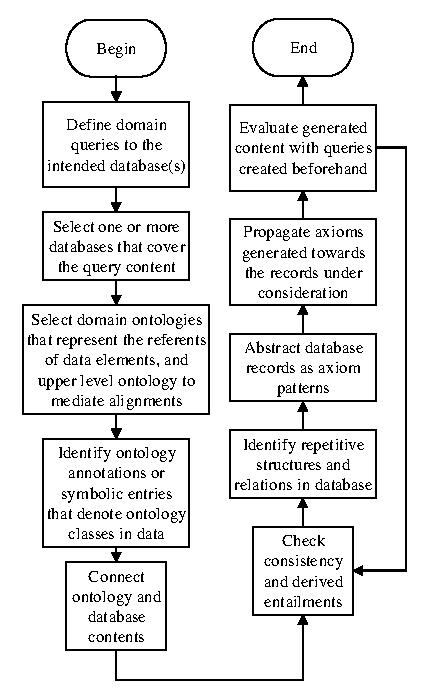
\includegraphics[width=0.65\linewidth]{PIC/process}
\caption{Ontology grounding process.}
\label{fig:process}
\end{figure}

For assessment and demonstration of the ontology grounding approach we have formulated the following CQs on Hcy metabolism. They explore database content concerning phenotypes, proteins, molecules and biological processes from several organisms, using ontologies and databases described in Section \ref{sec:resources}).

\begin{enumerate}
	\item Which kinds of biological processes related to Hcy can be found in mice?
	\item Which are the proteins that exhibit  \textit{methyltransferase activity}? 
	\item Which are the kinds of biological processes in which proteins of the type \textit{cystathionine gama lyase} participate, exhibiting \textit{carbon-sulfur lyase activity}?
	\item Which dysfunctional biological processes entail a risk of \textit{Myocardial infarction}?
	\item Which kinds of organisms are capable of performing `\textit{cysteine biosynthetic process}'?
	\item Which proteins found in ruminants have the capability of methionine biosynthesis? 
\end{enumerate}




\section*{Resources}
\subsection{Biomedical Ontologies}
\label{sec:onto}
%Annotations for biological processes, cellular components and molecular functions use GO. Protein and small molecule annotations use PR and ChEBI, respectively. In this work, GO, PR and ChEBI are organized under the BTL2 upper-level ontology. 
%As BTL2 is tailored to the biological domain, the alignment with ChEBI, PR and GO is facilitated. A brief description of each ontology is described below. 
%These ontologies are briefly characterised:\\
\begin{itemize}
	\item The \textbf{Gene Ontology} (GO) \citep{Gene2014a} was created in 1998 to address biomedical  information  integration through standardization of terms for the annotation of DNA sequences and their respective characteristics.  GO has become a crucial resource for functional genomics, as an ongoing collaborative effort that delivers a controlled vocabulary underpinned by an ontology language. GO provides class hierarchies under \textit{Cellular component}, \textit{Biological process}, and \textit{Molecular function} (ontologically better described as molecular activities or processes), together with relations between them.
	\item \textbf{Chemical Entities of Biological Interest} (ChEBI) \citep{Hastings2013} describes low-molecular-weight chemical entities for understanding and intervening in biological functioning. Each ChEBI entry denotes a chemical structure in a graphical form, together with ontological axioms. The ontology is subdivided into \textit{Molecular structure} and \textit{Biological role}. Whereas the former represents the structure of small molecules and their constituents, the latter is used to classify molecules depending on their disposition of participating in biological processes.
	\item The \textbf{Protein Ontology} (PR) \citep{Natale2014} is held by the Protein Information Resource (PIR), integrating several databases and responsible the current structure for the UniProt database. It represents modified forms, isoforms and protein complexes from living organisms and provides relations between them. 
	\item \textbf{SNOMED CT} \citep{IHTSDO2015} is a large clinical terminology for human and veterinary medicine, containing formal definitions, which can be expressed as an OWL-EL ontology. SNOMED CT covers clinical findings and disorders, body parts, devices, drugs, substances, organisms and clinical procedures, among others.  
	\item \textbf{BioTopLite 2} (BTL2)\citep{Schulz2013} is a lightweight and redesigned version of BioTop, created in 2006 as an upper-domain ontological layer to enable the representation of general aspects of biology and medicine. BTL2 offers highly constrained classes, using a small set of relations.  Classes like \textit{Organism}, \textit{Mono molecular entity}, and \textit{Body part} facilitate the alignment with other ontologies like GO, PR and ChEBI. BTL2 can be aligned with most of BFO and RO. Available biomedical ontologies compliant with these two sources can easily be integrated with BTL2.

\end{itemize}

\subsection{Biological Databases}
\label{sec:db}
\begin{itemize}
	\item The \textbf{Universal Protein Resource} (UniProt) \citep{UniProtConsortium2014} was created in order to enable a quick understanding of the field of proteomics. It provides a comprehensive, open-access resource of protein sequences and functional information. UniProt is mainly composed by a Knowledge Base (UniProtKB), subdivided in SwissProt (manually  curated) and TrEMBL (generated and maintained by automated tools). Other parts are databases for sequences, closely related protein sequences, protein information from fully sequenced organisms, and metagenomics. 	
	Data from literature and available in UniProt are organized and stored according protein and gene names, function, catalytic activity, cofactors, pathway information, sub-cellular location, among others. UniProt embeds NCBI Taxonomy identifiers directly throughout its structure, as well as GO annotations \citep{Huntley2014}, together with mappings to several biological databases including Ensembl.
	\item The \textbf{Ensembl} \citep{Cunningham2014} project was launched in 1999 in order to automatically annotate genomes and to integrate this data with other biological data sources, thus creating a freely available online source. Ensembl processes and summarizes large-scale genomic data for chordates and model organisms. Its content is related to the annotation of gene and transcript locations, gene sequence evolution, genome evolution, sequence and structural variants and regulatory elements. 
	\item The \textbf{NCBI Taxonomy} \citep{NCBI2015} was derived from a project on the taxonomy of biological organisms that aimed at extracting sequences not available in dedicated databases from genomic literature. This coincided with the collection of data about taxonomic classifications. The goal of NCBI Taxonomy is to combine existent, distributed organism taxonomies into a single one that is included in NCBI GenBank. 
\end{itemize}

\section*{Methods}
In the following, data acquisition and database conversion are described. Content and related files, such as spreadsheets, scripts, and ontology files can be downloaded from the project website (http://www.cin.ufpe.br/\~{}integrativo).

\subsection{Sampling} 
Data related to 21 species\footnote{Giant panda, Bovine, white-tufted marmoset, dog, zebrafish, chicken, human, West Indian ocean coelacanth, African elephant, mouse, European domestic ferret, Nile tilapia, rabbit, chimpanzee, Sumatran orangutan, rat, Tasmanian devil, pig, Japanese pufferfish. Western clawed frog}, together with processes and by-products related to Hcy metabolism are retrieved from the UniProt and Ensembl websites\footnote{UniProt: Release 2015\_04, Ensembl Release 79, NCBI Taxonomy 2015AA.}. The ontologies GO, ChEBI and BTL2 are downloaded in OWL2 format\footnote{GO Revision 25527, ChEBI Release 127, BTL2 Release 8th march 2015, PR release 22nd may 2015, SNOMED CT July 31st 2014.}. 

For the creation of a subset from UniProt and Ensembl, UniProt data are filtered by the string ``homocysteine'', thus retrieving all Hcy-related data from UniProt/SwissProt+Trembl. From the obtained  212,156 records the ones with GO annotations, specified gene names and proteins as described by \cite{Selhub1999} are selected. From the resulting 1,716 records fragments, isoforms, or homologue entries are excluded. 
The resulting set includes the proteins Methionine synthase (MS), Methylenetetrahydrofolate reductase (MTHFR), Cystathionine beta-synthase (CBS), and Gamma-cystathionase (CSE). After removing records without Ensembl IDs, a final sample with 46 Hcy-related records is made available as a Microsoft Excel spreadsheet with the following tabular structure:
\begin{itemize}
	\item One Protein (e.g. \textit{CBS)};
	\item One Taxon (e.g. \textit{Rattus norvegicus}); 
	\item One to many GO biological processes (e.g., \textit{Blood vessel remodeling}) 
	\item One to many GO molecular functions (e.g., \textit{CBS activity}) 
	\item One to many GO cellular components (e.g., \textit{Cytoplasm}) 
	\item Zero to many phenotypes (e.g., \textit{Endocrine pancreas increased size}) 	
\end{itemize}

\subsection{Ontology mappings}
Root classes from GO, PR, ChEBI, NCBI Taxonomy, and SNOMED CT are included as subclasses of BTL2 nodes and tested for logical consistency (Fig. \ref{fig:HierarquiaURI}).
%In particular,  
%\begin{enumerate}
%	\item One or more references to GO classes in UniProt annotations for GO classes, such as 
%go:`\textit{Biological process}' go:\textit{Methylation} included as annotation for `\textit{Methionine 
%synthase}' in UniProt, as well as go:`\textit{Cellular component}' and go:`\textit{Molecular function}';
%	\item Reference to Proteins from PR directly as protein names in UniProt;
%	\item Database IDs from Ensembl in UniProt, and vice-versa;
%	\item Organism names as described in NCBI Taxonomy inside Ensembl and UniProt;
%	%	\item Gene products (mainly proteins) described in UniProt and Ensembl and available in PR.
%	\item Phenotypes according to Ensembl and included as a list of subclasses of btl2:\textit{Situation}, 
%alinged with \textit{Clinical finding} in SNOMED CT.
%\end{enumerate}
%\subsection{Technical aspects for ontology grounding} 
%The grounding process requires in-depth biology knowledge, insight into the way biological databases are populated, as well as ontology engineering skills, based on the understanding of upper level ontology principles and description logics.
%
%Aware that a straightforward, automatized “ontologization” of a database schema is not possible, the ontology engineer has to critically assess the pros and cons of competing modelling strategies. This must be perfor- med in a way that correctly accounts for the underlying biological reality on the one hand, and that provides enough expressiveness to address the use cases (formulated as competency questions), on the other hand.
%
%The following technical aspects were applied:   
%\begin{itemize}%
%
%\item Top-level classes and relations of the domain ontologies were aligned manually with the upper level ontology (cf. \ref{fig:HierarquiaURI}) with the Protégé v5 beta 17 ontology editor;
Mapping consistency is assured with the DL reasoner HermiT 1.3.8. For performance optimization, modules of external ontologies (GO, ChEBI, PR and SNOMED CT) are created, with the classes 
referred to in the selected database content as signature, using the Prot\'{e}g\'{e} plug-in Ontology Modularity \citep{Jiang2011}.  

All database objects are subjected to in-depth ontological analysis done by the authors. The content of a representative 
sample record is entirely modelled in Prot\'{e}g\'{e} as an OWL ontology, and tested for consistency and adequacy under BTL2. Once agreement is reached, this sample ontology is saved in OWL/XML format and manually dissected into code fragments, each of which is numbered and placed into a spreadsheet cell.  The code fragments are analysed to identify variable elements, i.e. class names specific to the underlying sample, encompassing protein, cellular component, biological function and other classes. All these names are then replaced by placeholders, thus yielding an ontology pattern specific to the data structure. 
The target ontology is then generated by iteratively filling the placeholders with the ontology class names from the database. This is done using a customized VBA script. This script has to account for the creation of named subclasses as well as for iterations over content of multi-valued fields.  

%

\subsection{Evaluation methodology} \label{EvaluationMethodology}
The ontological content is evaluated by six competency questions (CQs),as introduced above. Formulated in English by the first author, a biologist, they are shaped according to how domain experts would query a biological database, and not how ontology engineers would interpret it, in order to be neutral regarding the internal structure of the ontology.
The translation of CQs into DL queries relies on the correct identification of query components that denote relations, referents, and the way how domain entities are related to one another (cf. section \ref{section:CQ}). To avoid biased judgements, this process is assessed by means of DL 
classification and retrieval of content from the axioms generated. %This is possible as CQs 
are rendered as DL queries and submitted to the final ontology.

 
Scalability is evaluated by artificially increasing the size of the ontology by a scaling factor $f$ $\in$ {1, 3, 10, and 30}. This is done programmatically, creating new classes suffixed by $i$ $\in$ {1, 2, \ldots, $f$}. Tangledness of these experimental ontologies is guaranteed by random assignment of \textit{i} in the axioms.  
The resulting ontologies are submitted to a DL reasoner to verify classification time. In addition, 
satisfiability time is measured, defined as the time it takes for validating a CQ 
against the derived model from the test ontology.
All tests are performed in Intel core i7-4510U laptop, with 8Gbytes of RAM, running Windows 10 (x64) and Java 8 (update 66, x64).


\section*{Results}
\begin{table*}[t]
	\begin{threeparttable}
		\caption{Uniprot and Ensembl table view}
		\label{table:uniprot}
		\centering
		\begin{tabular}{p{0.45in}p{0.4in}p{0.5in}p{0.8in}p{0.8in}p{0.6in}|p{1.25in}p{1.2in}} 
			\hline 
			Entry & Protein & Organism & GO (bp) & GO (mf) & GO (cc) & Ensembl ID & Ensembl Phenotype\\ \hline 
			F1MEW4 & CBS & \textit{Bos taurus} & blood vessel remodeling; \ldots & cystathionine $\beta$-synthase activity \ldots & cytoplasm \ldots & ENSBTAT00000000184; \ldots & No phenotype associated \\ 
			Q99707 & MS & \textit{Homo sapiens} & cobalamin metabolic process; \ldots & cobalamin binding; \ldots & cytoplasm \ldots & ENST00000366577; ENST00000535889 & Neural tube defect; Megaloblastic anemia; \ldots \\ \hline 
		\end{tabular}
		\begin{tablenotes}
			\item The left six columns contain UniProt entries; the two right columns correspond to Ensembl in entried. GO (bp) , GO (mf) and GO (cc) represents rows from UniProt that include annotations for GO classes '\textit{Biological process}', '\textit{Molecular function}' (understood as activity) and '\textit{Cellular component}'. IDs from UniProt and Ensembl are used for mapping purposes.\\ 
		\end{tablenotes}
	\end{threeparttable}
\end{table*}
 
\begin{table*}[t]
	\centering
	\caption{Template table}
	\label{table:template}
	\begin{tabular}{p{0.3in}p{0.3in}p{0.3in}p{0.6in}p{0.6in}p{0.6in}p{0.6in}p{0.6in}} \hline 
		\# & \textit{P} &\textit{O} & \textit{Bp} & \textit{Mf} & \textit{C} & \textit{Ph} & \textit{M} \\ \hline 
		$k$ & $P_k$ & $O_k$ & $Bp_1\ldots n$ & $Mf_1\ldots n$ & $C_1\ldots n$ & $Ph1\ldots n$ & $M_1\ldots n$ \\
		\ldots & \ldots & \ldots & \ldots & \ldots & \ldots & \ldots & \ldots \\
		$l$ & $P_l$ & $O_l$ & $Bp_1\ldots n$ & $Mf_1\ldots n$ & $C_1\ldots n$ & $Ph1\ldots n$ & $M_1\ldots n$ \\
		\ldots & \ldots & \ldots & \ldots & \ldots & \ldots & \ldots & \ldots \\
		$m$ & $P_m$ & $O_m$ & $Bp_1\ldots n$ & $Mf_1\ldots n$ & $C_1\ldots n$ & $Ph1\ldots n$ & $M_1\ldots n$ \\ \hline 
	\end{tabular}
	\begin{tablenotes}
		\item The symbol \# represents record IDs; \textit{P} proteins; \textit{G} genes; \textit{O} organisms; \textit{Bp} biological processes;
		\textit{Mf} molecular function; \textit{C} cellular component; \textit{Ph} phenotype; and \textit{M} the associate molecules. \\ \\
	\end{tablenotes}
\end{table*}

\subsection{Basic ontological assumptions}
The thorough inspection of the database (DB) content and its discussion among the authors yielded the following ontology-based interpretation: ``Each DB record can be understood as introducing a series of defined subclasses of each biological process class referred to by this DB record. Each of these subclasses is defined by having one or more proteins of a certain type as participants, together with the small molecule Hcy. These proteins occur within one or more cell components. If dysfunctional, these processes lead to the risk of developing the pathological phenotypes mentioned in the source".

Thus, the content of the biological database extract under scrutiny is entirely expressed at class level. The underlying assumption is that all these defined process subclasses are non-empty, as otherwise there would not have been any experimental evidence manifested as a curated database entry. Additionally, we assume that no wrong data occur (data instances that do not have any referent in reality). This interpretation allows us to refrain from reasoning about individuals, thus avoiding scaling problems.  

%E.g. reasoning is used to classify and check consistency of classes, which in turn are used to enable relations among individuals. Considering relationships among individuals are limited by the relations from class description, and in most use case scenarios 7 individuals must follow their class -based descriptions, all consistency checking and classification may be performed only according the T-box. This avoid the high computational cost of reasoning with A-box individuals.
%
%With our interpretation, a record subtlety is represented   as a new subclass. In other words, a record that introduces a human being able to develop diabetes due to high sugar diet is a type of human that reacts to a high sugar diet as being able to develop diabetes. This approach, at the same time, is able to represent ontologically the record content and do not entail performance issues. Thus, avoid the creation of misleading class definitions to commit to the world interpretation embedded on data.
%
%The construction of the appropriate ontology pattern had to consider several implicit facts. Apart from the general assumption that Hcy takes place in all of the described processes, we have to assert that the they are related to both cell components and organisms via the BTL2 relation `\textbf{is included in}', and that only dysfunctional processes lead to the risk of developing certain pathological phenotypes.

%Each record from UniProt and Ensembl is interpreted as unique; one or more similar experiments may have resulted in the population of a single DB record. 


\subsection{Ontological Grounding}

In the following, the ontological grounding steps of the selected content is described. 
%In addition, we present one example use case. 
%
%\subsection{Evaluating data}
Table \ref{table:uniprot}) shows a subset of the table created as a view from UniProt and Ensembl (Table \ref{table:uniprot}). We translate the content from table \ref{table:uniprot} as an example table \ref{table:template} for interpretation. 
As a first task, we determine the ontological representation of data in Table \ref{table:template}: 

\begin{itemize}
	\item There exist biological processes of the type \textit{Bp} in organisms of the type \textit{O} that have the protein \textit{P} and the small molecule \textit{M} as participants;
	\item In each \textit{Bp}, the protein \textit{P} is capable of performing one or more molecular functions (processes) \textit{Mf} ;
	\item \textit{Bp} processes  occur in one or more types of cellular components \textit{C};
	\item There exist biological processes of the type \textit{Bp} that are dysfunctional and therefore bear the risks of causing one or more pathological phenotypes of the type \textit{Ph};
	\item All organisms of the type \textit{O} have dispositions to be realized by \textit{Bp} processes;
	\item All types of protein \textit{P} in \textit{O} are able to perform \textit{Mf} processes;
	\item Proteins of class \textit{P} are not organism-specific. However, as the DB records refer to organism-specific proteins we introduce subclasses \textit{P\_sensu\_O} for each DB record (Protein \textit{P} from Organism type \textit{O}).
	\item Each \textit{Bp} referred to by in a DB record may happen within the same cellular structure in several organisms \textit{O}, including organism-specific proteins \textit{P} and molecules \textit{M}. However, each DB record denotes an exclusive occurrence of \textit{Bp}. In this sense, each DB record is interpreted as denoting specific subclasses of \textit{Bp}, identified as \textit{Bp\_in\_O\_with\_P\_and\_M}, generated as a combination of biological process, organism, protein and small molecule; 
	\item The database structure leaves open in which cellular component \textit{C} a given \textit{Bp} subclass is located, when there is more than one entry in the cellular component field. For this reason, we generate union classes of the type $C_1$ or $C_2$ or \ldots or $C_n$ to which the process locations can be safely assigned.
	\item The DB structure is not explicit enough to connect a \textit{Bp} subclass to a specific \textit{Mf} process. Therefore in the definition of each \textit{Bp} subclass the \textit{Mf} processes are attached to the protein agent of that \textit{Bp} subclass as possible realisations of the related disposition class (`\textbf{is realized by}' only \textit{Mf}); 
	\item If there are phenotype entries \textit{Ph}, a new class of the type \textit{Dysfunctional\_Bp\_in\_O\_with\_P\_and\_M} is generated for every \textit{ Bp\_in\_O\_with\_P\_and\_M}, and all phenotypes are referred to as being the realizations of risks.
\end{itemize}

With this strategy, process subclasses appear in query results, which may appear confusing for the user, who only expects the parent classes from which they are derived, i.e. biological process classes from GO, as they exist as entries in database records. 
% I REMOVED THE FOLLOWING. THE READER WOULD WONDER WHAT VIRTUAL CLASSES ARE
%These subclasses represent content from records. Considering that (i) 
%classes generated from data are virtual classes, and (ii) virtual classes 
%are specific occurrences of a given class, the user may want to know the real ones. In these case, it is %required to verify and group to which classes the ones denoted belong. 
%
%Examples are delivered together with CQs in Section \ref{section:CQ}.
%In all cases, when querying any ontology derived from an interpretation process like this, we must perform a two step query. 
This is the reason why the query results need to be post-processed in a way that only the original superclasses are filtered out. E.g., 
if the class \textit{BpX\_in\_O\_with\_P\_and\_M} is retrieved by the query, only its superclass \textit{BpX} is displayed. 

\subsection{Ontology patterns}

This analysis allows us to identify ontology patterns. First, we present the definitions of \textit{P}(table \ref{table:ProteinP}), \textit{Bp} (table \ref{table:Bp}) and \textit{C} (table \ref{table:CellCompC}). 

Table \ref{table:ProteinP} shows how organism-specific proteins types \textit{P} are introduced as defined subclasses of pr:\textit{Protein}.

\begin{table}[H]
	\caption{Defined subclasses of proteins $P$}
	\label{table:ProteinP}
	\centering
	\begin{tabular}{c}
		\hline
		\textit{P\_sensu\_O} equivalentTo \textit{P} and (`\textbf{is included in}' some \textit{O}) \\
		\textit{P} subclassOf pr:\textit{Protein} \\ 
		\textit{P\_sensu\_O} subclassOf \textit{P} \\
		\hline
	\end{tabular}
\end{table}%
\noindent
 The composed name denotes a species-specific protein class: \textit{P\_sensu\_O} is a sublass of \textit{P}.

\begin{table}[H]
	\caption{Defined subclasses of biological process $Bp$}
	\label{table:Bp}
	\centering
	\begin{tabular}{p{3in}}
		\hline
			\textit{Bp} subclassOf go:`\textit{Biological process}' \\
			\textit{\textit{Bp}\_in\_O\_with\_P\_and\_M} subclassOf \textit{Bp} \\
			\textit{Dysfunctional\_Bp\_in\_O\_with\_P\_and\_M} subclassOf  \\
			\hspace{1cm} \textit{Bp\_in\_O\_with\_P\_and\_M} \\
		\hline
	\end{tabular}
\end{table}%

\noindent
Biological processes \textit{Bp} are subclasses of the GO class \textit{Biological process}, and the mention of a specific biological process in a database entry in the context of a specific organism, a specific protein, and a specific small molecule determines the creation of the class \textit{Bp\_in\_O\_with\_P\_and\_M} as subclass of \textit{Bp}.

Cellular components of any type $C$ (within a single DB record) are defined as subclasses of the GO class \textit{Cellular component} (Table \ref{table:CellCompC}).

\begin{table}[H]
	\caption{Cellular component $C$ union classes}
	\label{table:CellCompC}
	\centering
	\begin{tabular}{p{3in}}
		\hline
		\textit{$C_1\_or\_C_2\_or\_\ldots\_or\_C_n$} subclassOf go:`\textit{Cellular component}' \\
		{$C_1\_or\_C_2\_or\_\ldots\_or\_C_n$} equivalentTo $C_1$ or $C_2$ or \ldots or $C_n$ \\
		\hline
	\end{tabular}
\end{table}%
\noindent
 When a record refers to more than one cellular component class, union classes type $C_1$ or $C_2$ or \ldots or $C_n$ are created under the GO class \textit{Cellular component}. This is due to the fact that the DB structure is not explicit enough to connect specific cellular components to specific process subclasses.

Table \ref{table:BpComposite} shows the axioms for \textit{Bp\_in\_O\_with\_P\_and\_M} classes.

\begin{table}[H]
	\caption{$Bp\_in\_O\_with\_P\_and\_M$}
	\label{table:BpComposite}
	\centering
	\begin{tabular}{p{3in}}
		\hline
		 \textit{Bp\_in\_O\_with\_P\_and\_M} equivalentTo \textit{Bp}\\\
		\hspace{0.5cm} and (`\textbf{has participant}' some \textit{M})\\
		\hspace{0.5cm} and (`\textbf{has participant}' some \\
		\hspace{1cm}(\textit{P} and (`\textbf{is bearer of}' some (btl2:\textit{Function} and \\
			\hspace{1.5cm} (`\textbf{is realization of}' only \textit{Mf}))) \\
			\hspace{0.5cm} and (`\textbf{is included in}' some ($C_1$ or $C_2$ or \ldots or $C_n$)) \\
			\hspace{0.5cm} and (`\textbf{is included in}' some \textit{O}) \\
\hline
	\end{tabular}
\end{table}
\noindent
Axioms for \textit{Bp\_in\_O\_with\_P\_and\_M} (Table \ref{table:BpComposite}) describe that a biological process from a single record has one or more small molecules as participants; the process is included in the combination of one or more cellular components within organism of a specific species; and the protein from the record is a participant in the process, and has the function of performing molecular processes of certain types.

Some \textit{Bp\_in\_O\_with\_P\_and\_M} processes are dysfunctional and therefore entail the risk of pathological phenotypes (represented as SNOMED CT findings, ontologically subclasses of btl2:\textit{situation}).

\begin{table}[H]
	\caption{Dysfunctional phenotypes of $Bp\_in\_O\_with\_P\_and\_M$}
	\label{table:DysfunctionalBpComposite}
	\centering
	\begin{tabular}{p{3in}}
		\hline
		\textit{Dysfunctional\_Bp\_in\_O\_with\_P\_and\_M} equivalentTo \\ \hspace{0,5cm}\textit{Bp\_in\_O\_with\_P\_and\_M} \\
		\hspace{1cm} and (`\textbf{is bearer of}'  some `\textit{Dysfunctional Quality}') \\
		\textit{Dysfunctional\_Bp\_in\_O\_with\_P\_and\_M} subClassOf \\
		\hspace{0.5cm} \textit{Bp\_in\_O\_with\_P\_and\_M} \\
		\hspace{1cm} and (`\textbf{is realization of}' only (\textit{Risk} and (\textbf{causes}  some \textit{Ph}))) \\
		\hline
	\end{tabular}
\end{table}%
\noindent
\textit{Dysfunctional\_Bp\_in\_O\_with\_P\_and\_M} are processes defined by the quality of being dysfunctional. They are realizations of the risk (a sort of disposition) of causing the dysfunctional phenotype stated in the DB.

Table \ref{table:PComposite} presents the axioms required to represent \textit{P\_sensu\_O}, i.e. the species-specific class of proteins \textit{P}.

\begin{table}[H]
	\caption{Subclasses created for the organism specific protein ($P\_sensu\_O$) classes in database records}
	\label{table:PComposite}
	\centering
	\begin{tabular}{p{3in}}
		\hline
\textit{P\_sensu\_O} equivalentTo \textit{P} and (`\textbf{is included in}' some \textit{O}) \\
\textit{P\_sensu\_O} subClassOf \textit{P} and (`\textbf{is bearer of}'  some (\textit{Function} and \\			
\hspace{1cm} (`\textbf{has realization}' only \textit{Mf}))) \\
		\hline
	\end{tabular}
\end{table}%
\noindent
Definitions that follow the pattern from Table \ref{table:PComposite} describe organism-specific protein molecule classes. In addition, the \textit{Mf} processes specified in the DB records are added. 
%Note that we interpret all content of the GO molecular function branch as processes, hence the reference to them via the `\textbf{has realization}' relation. 

The last axiom required is about organisms as bearers of dispositions related to performing biological processes (Table \ref{table:Organism}) .

\begin{table}[H]
	\caption{Axioms generated for organisms  $O$ in database records}
	\label{table:Organism}
	\centering
	\begin{tabular}{p{3in}}
		\hline
			\textit{O} subClassOf btl2:\textit{Organism} and \\
			\hspace{0.5cm} (`\textbf{is bearer of}'  some (\textit{Disposition} and \\
			\hspace{1cm} `\textbf{has realization}' only \textit{Bp}))) \\
		\hline
	\end{tabular}
\end{table}%
\noindent
Table \ref{table:Organism} attaches dispositions realized by specific biological processes to organisms. 

\subsection{Evaluating the content generated}
\label{sec:evaluation}
The analysis of the content of database entries has resulted in a set of OWL T-Box axioms for each database record as specified above. We recall two basic assumptions made, \textit{viz.} (i) non-emptiness of classes: i.e. each of the newly defined classed corresponds to at least one fact described in literature, and (ii) the veracity of database entries, i.e. each information is considered a statement of truth. Given these boundary conditions, evaluation of the generated TBoxes will address the aspects: (i) logical satisfiability when importing all constraints from the upper-level-ontology BTL2; (ii) adequacy (correctness and completeness) of entailments against CQs; and, (iii) computational performance.

%\subsubsection{Evaluation of Satisfiability}
%This step is evaluated automatically with the support of HermiT OWL2 reasoner. When a new version of the ontology is created and new subclasses are generated from records, the reasoner is used to verify if the content is satisfiable (logically sound). To exemplify the procedure, we evaluate with the reasoner if a class of the type \textit{Bp\_in\_O\_with\_P\_and\_M} is (or is not) equivalent to the original \textit{Bp} superclass. To be more specific, such as if `\textit{methylation\_in\_Homo\_sapiens\_with\_Methionine\_synthase\_and\_Homocysteine}' is a \textit{methylation}. 
%
%Other type of logical satisfiability performed is the evaluation of the correct usage of relations inside the axioms created, for instance, when applying the relation `\textbf{has realization}' between an organism of the type \textit{O} and a biological process of type \textit{Bp}. According to BTL2, material entities are bearers of the capability (\textit{Role}, \textit{Function} or \textit{Disposition}) that culminates with the realization of a specific process.

\subsubsection{Evaluation of Competency Questions (CQs)}
\label{section:CQ}
In the following, each competency question is translated into a DL query. The result is analysed and discussed.  

\paragraph{CQ1:	Which kinds of biological processes related to Hcy can be found in mice? (Table \ref{table:cq1})}
This query is intended to retrieve all biological process classes that takes place in organisms.  
%The relevance of this query regards the retrieval of the biological processes available in data for the specific organism mentioned.

\begin{table}[H]
	\caption{Competency Question CQ1 in DL}
	\centering
	\label{table:cq1}
	\begin{tabular}{p{3in}}
		\hline
			`\textit{Biological process}' and `\textbf{is included in}'  some `\textit{Mus musculus}' \\
		\hline
	\end{tabular} 
\end{table}

34 subclasses (including ancestors) are retrieved. After filtering out the system-defined subclasses we obtain: \textit{Amino acid betaine catabolic process}, \textit{Blood vessel remodeling}, \textit{Cellular response to hypoxia}, and other 31 biological processes. The results are expected 
as they correspond to the content of the database.

\paragraph{CQ2: Which are the proteins that exhibit \textit{methyltransferase activity}?  (Table \ref{table:CQ2})}
This query is meant to retrieve classes of proteins that are able to perform certain \textit{Mf} processes. It is important that some proteins are capable to act in a specific way, like polymorphisms in gene MS leads to methionine synthase deficiency, which leads to higher Hcy levels together with dysfunctional phenotypes in humans and mice. 
\begin{table}[H]
	\caption{Competency Question CQ2 in DL}
	\centering
	\label{table:CQ2}

\begin{tabular}{p{3in}}
	\hline  
		\textit{Protein} and (`\textbf{is bearer of}' some \textit{Function} and \\
		\hspace{0.5cm} (`\textbf{has realization}' only `\textit{Methyltransferase activity}')) \\ 
	\hline 
\end{tabular} 
\end{table}

38 subclasses (including ancestors) are retrieved. After filtering out the system-defined subclasses we obtain: \textit{Betaine homocysteine S methyltransferase 1}, \textit{Cystathionine beta synthase}, \textit{Cystathionine gamma lyase}, \textit{Cystathionine gamma lyase}, \textit{Methionine synthase}, and \textit{Methylenetetrahydrofolate reductase}. These five protein classes, which have the ablility to perform the process \textit{Methyltransferase activity} correspond to the database content.

\paragraph{CQ3: Which are the kinds of biological processes in which proteins of the type \textit{cystationine gamma lyase} participate, exhibiting \textit{carbon-sulfur lyase activity}? ( Table \ref{table:cq3})}
This query is related to the identification of biological processes (e.g. biochemical reactions) that involve a specific protein (enzyme), which should play a role in this reaction. The relevance of this query is related to the capability of retrieving specific biological processes by means of reaction-specific proteins . 
\begin{table}[H]
	\caption{Competency Question CQ3 in DL}
	\label{table:cq3}
		\centering
	\begin{tabular}{p{3in}}
		\hline
			`\textit{Biological process}' and \\
			\hspace{0.5cm} `\textbf{has participant}'  some (`\textit{Cystationine gamma lyase}' and \\
			\hspace{1cm} (`\textbf{is bearer of}'  some (\textit{Function} and (`\textbf{has realization}'  only \\
			\hspace{2cm} `\textit{Carbon-sulfur lyase activity}'))))) \\
		\hline
	\end{tabular} 
\end{table}

34 subclasses (including ancestors) are retrieved. After filtering out system-defined subclasses, the following eleven remain: \textit{Cellular nitrogen compound metabolic process}, \textit{Cysteine biosynthetic process}, \textit{Endoplasmic reticulum unfolded protein response}, \textit{Hydrogen sulfide biosynthetic process}, \textit{Negative regulation of apoptotic process}, \textit{Negative regulation of apoptotic signaling pathway}, \textit{Positive regulation of I kappaB kinase NF kappaB signalling}, \textit{Protein homotetramerization}, \textit{Protein pyridoxal phosphate linkage via peptidyl N pyridoxal phosphate L lysine}, \textit{protein sulfhydration}, and \textit{small molecule metabolic process}.

	%
	%Below, the results.
	%
	%\begin{itemize}
	%	\item [--]Results:
	%		\begin{itemize}
	%			\item `\textit{cellular nitrogen compound metabolic process in Homo sapiens with cystathionine gamma lyase and Homocysteine}';
	%			\item `\textit{cysteine biosynthetic process in Homo sapiens with Cystathionine gamma lyase and Homocysteine}';
	%			\item and 32 more classes.
	%		\end{itemize}
	%\end{itemize}

\paragraph{CQ4: Which dysfunctional biological processes entail a risk of \textit{Myocardial infarction}?  (Table \ref{table:cq4})}

%This query retrieves biological processes that are associated with the risk of developing a dysfunctional phenotype. This query is relevant as it helps identify pathological phenomena associated with a specific biological process.
%\begin{table}[H]
%	\caption{Competency Question CQ4}
%	\label{table:cq4}
%		\centering
%	\begin{tabular}{p{3in}}
%		\hline
%			`\textit{biological\_process}' and (`\textbf{is realization of}' only \\ 
%			\hspace{1cm}(\textit{Risk} and (\textbf{causes}  some `\textit{Vascular sclerosis}'))) \\
%		\hline
%	\end{tabular} 
%\end{table}
%
%Ten classes (including ancestors) are retrieved: \textit{Dysfunctional homocysteine metabolic process}, \textit{Dysfunctional methionine biosynthetic process}, \textit{Dysfunctional one carbon metabolic metabolic}, \textit{Dysfunctional response to amino amino}, \textit{Dysfunctional response to drug}, \textit{Dysfunctional response to hypoxia}, \textit{Dysfunctional response to interleukin interleukin}, \textit{Dysfunctional response to vitamin }, \textit{Dysfunctional S adenosylmethionine metabolic metabolic}, and \textit{Dysfunctional tetrahydrofolate metabolic process}. None of these processes is related in the database with the entry \textit{Vascular sclerosis}, but they are correctly retrieved because they are related to \textit{Atherosclerosis}, which is a subclass of \textit{Vascular sclerosis} in SNOMED CT. 

%%%%% TRECHO COMENTADO REFERE-SE AO CONTEÚDO MODIFICADO DA CQ4 DESCRITO NO EMAIL. BASTA DESCOMENTAR. O CONTEÚDO DA RESPOSTA É EXATAMENTE IGUAL!!

This query retrieves biological processes that are associated with the risk of developing a dysfunctional phenotype. This query is relevant as it helps identify pathological phenomena associated with a specific biological process.
\begin{table}[H]
	\caption{Competency Question CQ4}
	\label{table:cq4}
	\centering
	\begin{tabular}{p{3in}}
		\hline
		`\textit{Biological process}' and (`\textbf{is realization of}' only \\ 
		\hspace{1cm}(\textit{Risk} and (\textbf{causes} some `\textit{Myocardial infarction}'))) \\
		\hline
	\end{tabular} 
\end{table}

Ten classes (including ancestors) are retrieved: \textit{Dysfunctional homocysteine metabolic process}, \textit{Dysfunctional methionine biosynthetic process}, \textit{Dysfunctional one carbon metabolic metabolic}, \textit{Dysfunctional response to amino acid}, \textit{Dysfunctional response to drug}, \textit{Dysfunctional response to hypoxia}, \textit{Dysfunctional response to interleukin 1}, \textit{Dysfunctional response to vitamin B2}, \textit{Dysfunctional S adenosylmethionine metabolic process}, and \textit{Dysfunctional tetrahydrofolate metabolic process}. None of these processes is related in the database with the entry \textit{Myocardial infarctation}, but they are correctly retrieved because they are related to \textit{Acute myocardial infarction of anterior wall}, which is a subclass of \textit{Myocardial infarction} in SNOMED CT. 

\paragraph{CQ5: Which kinds of organisms are capable of performing cysteine biosynthesis?  (Table \ref{table:cq5})}
This query retrieves organisms that are capable of performing specific biological processes. This query is relevant because not all biological processes for organisms are fully described. Organisms from different species that include for which the same proteins under the same conditions are described  may not include similar processes
\begin{table}[h!]
	\caption{Competency Question CQ5}
	\label{table:cq5}
		\centering
	\begin{tabular}{p{3in}}
		\hline
			\textit{Organism} and (`\textbf{is bearer of}'  some (\textit{Disposition} and \\
			\hspace{1cm} (`\textbf{has realization}' only \textit`\textit{Cysteine biosynthetic process}'))) \\
		\hline
	\end{tabular} 
\end{table}

The following organism classes were retrieved: \textit{Ailuropoda melanoleuca}, \textit{Bos taurus}, \textit{Callithrix jacchus}, \textit{Danio rerio}, \textit{Gallus gallus}, \textit{Homo sapiens}, \textit{Latimeria chalumnae}, \textit{Loxodonta africana}, \textit{Mus musculus}, \textit{Mustela putorius furo}, \textit{Oreochromis niloticus}, \textit{Oryctolagus cuniculus}, \textit{Pan troglodytes}, \textit{Rattus norvegicus}, \textit{Sarcophilus harrisii} and \textit{Takifugu rubripes}.

\paragraph{CQ6: Which proteins found in ruminants have the capability of methionine biosynthesis? (Table \ref{table:CQ6})} 
The aim of this query is to retrieve specific proteins that are related to the process \textit{methionine biosynthetic process}, when performed by a organism of the suborder \textit{Ruminantia}. In other words, we are able to identify specific proteins by means of organisms and biological processes among the content embedded in databases.
\begin{table} [H]
		\label{table:CQ6}
		\caption{Competency Question CQ6}
		\centering
\begin{tabular}{p{3in}}
	\hline 
		\textit{Protein} and (`\textbf{is included in}' some (\textit{Ruminantia} and \\
		\hspace{0,5cm}(`\textbf{is bearer of}' some (\textit{Disposition} and (`\textbf{has realization}' only \\
		\hspace{1cm} `\textit{Methionine biosynthetic process}')))) \\ 
	\hline 
\end{tabular} 

\end{table}
Five subclasses (including ancestors) are retrieved, of which the following are displayed after filtering:  \textit{Betaine  homocysteine S methyltransferase 1}, \textit{Cystathionine beta synthase}, \textit{Cystathionine gamma lyase}, \textit{Methionine synthase}, and \textit{Methilenetetrahydrofolate reductase}. Although the entry \textit{Ruminantia} is not found in the database source, the result is correct, because all entries refer to \textit{Bos taurus}, which is a subclass of \textit{Ruminantia} in the NCBI taxonomy.

%The results from CQ6 are displayed below.
%
%\begin{itemize}
%	\item Result: 
%	\begin{itemize}
%		\item `\textit{Betaine homocysteine S-methyltransferase 1 sensu Bos taurus}';
%		\item `\textit{Cystathionine beta synthase sensu Bos taurus}';
%		\item and 3 more classes.
%	\end{itemize}
%\end{itemize}

%%%%%%%%%%%%%%%%%%%%%%%%%%%%%%%%%%%%%%%%%%%%%%%%%%%%%%%%%%%%%%%%%%%%%%%%%%%%%%%%%%%%%%%%%%
%
%%This table appears only in section 5.4.3 - Computational Performance
\begin{table*}[t]
	\begin{minipage}{\textwidth}
		\label{table:Summary}
		\caption{Survey of ontology sources, expressivity and reasoning performance in milliseconds}
		\centering
		\begin{tabular}{lrrrcrrrrrrrrr}
			\hline Ontology & Classes & Subcl. Axioms & Eq. Axioms & DL & Classification (h) & CQ1 & CQ2 & CQ3 & CQ4 & CQ5 & CQ6 \\ 
			x1  &  903 & 1,053  & 647 & $ALC$  & 586ms & 8ms & 13ms & 31ms & 35ms & 39ms  & 44ms \\ 
			x3 &  2,512 	& 2,957 & 1,945 & $ALC$  & 3,831ms & 12ms & 16ms & 32ms &  33ms & 38ms  &  39ms \\ 
			x10  & 8,599	 &  10,268 & 6,707 & $ALC$ & 38,994ms &70ms & 75ms & 85ms & 88ms & 92ms & 93ms \\ 
			%x30  & 25945 & 31072 & 20398 & $ALC$ & 397006ms  & 0ms & 1ms & 5ms  & 6ms  & ms &  ms  \\ 
			Modularized  & 2,838  & 4,071 & 1,203 & $SRI$ & 7,233,529ms & 373ms & 381ms & 385ms & 394ms & 397ms & 402ms \\ 
			\hline 
		\end{tabular} 
	\end{minipage}
\end{table*}


\subsubsection{Computational performance}
%output of the ontology grounding process is a OWL file with  
%the interpreted axioms propagated towards the   %%%% PROPAGATE ?? DON'T UNDERSTAND
%database or database subpart. 
In order to evaluate the computational costs of our approach, we compare the generated and mapped ontologies with an upscaled, artificially generated ontology having the same configuration.

Table 16 presents the reasoning performance of these OWL files with the queries CQ1-CQ6. It shows that under DL expressivity $ALC$  classification time increases proportionally with the number of classes and axioms, without sacrificing satisfiability of queries and the retrieval of classes. 

With the increase of expressivity from $ALC$ to $SRI$ (inherited from BTL2), reasoning time amounts to approximately two hours for classification and consistency checking. Thus, CQ satisfiability time also increases, but keeps performance in a reasonable time, i.e. not more than half a second. 


%%%%%%%%%%%%%%%%%%%%%%%%%%%%%%%%%%%%%%%%%%%%%%%%%%%%%%%%%%%%%%%%%%%%%%%%%%%%%%%%%%%%%%%%%%%%%%%
%
%



\section*{Discussion}
The focus of this work is the formal interpretation of biological database content with the goal to enable content retrieval using powerful ontology-based queries.
We demonstrated the ability of OWL ontologies using description logics reasoning to retrieve statements of interest from biological databases. 

We implemented and tested a use case based on database extracts describing amino acid metabolism. 
The interpretation is based on a specific ontological interpretation of representing biological database content: From each database record numerous defined OWL classes are generated, covering proteins, processes, molecular activities and dysfunctional phenotypes. Each class is assumed to contain at least one individual entity, corresponding to the outcome of a specific biological experiment described in the database. These individuals, however, are not explicitly represented in the ontology, as little as the data individuals in the database, which denote the domain entities.    
Thus, all content is exclusively represented in a Tbox, which warrants finite and complete reasoning, in contrast to the costs of rich TBoxes together with populated ABoxes \citep{Motik2006a}. 


%We ontologically ground database content, submitting the  generated 
%content to a formal scrutiny. The process is guided by ontological 
%principles and CQs written in DL.

% This view can be updated with according to the queries created. 
%However, the ontological interpretation of the database 
%does not entail changes, e.g. due to the fixed database organization. In other 
%words, the interpretation given to "what is a protein" from a single database may vary only if its schema changes. 

The output, an ``ontologized'' database representation, enables queries on the experimental results summarized in database records. 
The fact that typical queries often target possibilities ``\textit{Are members of the class A able to do B}?'' is addressed by two mechanisms. Firstly, by the inclusion of dispositions and functions as first-class entities in our ontology (as provided by the upper-level ontology BTL2), and secondly by the above mentioned addition of specific subclasses, assuming that these subclasses are  
populated. An example: the fact that our generation approach creates the class 
\textit{Cellular nitrogen compound metabolic process in Homo sapiens with Betaine homocysteine S methyltransferase 1 and Homocysteine}, which is created as a defined subclass of the GO class 0034641 (\textit{Cellular nitrogen compound metabolic process}), means that this process has been described at least once for Human with Homocystein and the related enzyme.  
%, i.e. there are database records that support the creation of one or more classes. 
In this sense, the question ``Are members of the class $A$ able to do $B$?" boils down to the question ``Does $A$ have a subclass $A'$ all members of which actually do $B$?''
%, to highlight the existence of classes, and not its direct assertion. 

Interpreting database content under an ontological perspective has been a topic of research interest \citep{Lehmann2009,Kanehisa2012,Carnielli2015}. 
%\cite{Fanizzi2008} present a tool called DL- FOIL, which relies on refinement operators for class-learning. In DL-FOIL grounding is presented as learning by search of class definitions in an induced search space. A limitation of DL-FOIL is the treatment of individuals that do not belong to a specific class, as well as the incompleteness of the refinement operator.
The DL-Learner system \cite{Lehmann2009} is grounded on the requirement for schema acquisition methods, addressed by class learning techniques. DL-Learner is designed to find logical explanations for individuals. It is limited by the fact that positive and negative examples must be provided, and individuals must be included directly in the ontology.
In the biomedical domain, \cite{Kanehisa2012} highlighted the importance of data interpretation from biomedical databases. Interpretation strategies are embedded in KEGG by a set of mapping operations among internal modules, allowing the identification of organism-specific pathways. QueryGen \citep{Bobed2016} presented a system that, given user keywords, proposes formal queries to retrieve data from repositories. 
% I REMOVED THE NEXT SENTENCE AS IST IS NOT UNDERSTANDABLE
%In comparison, our approach already performs this task beforehand when the user interprets the database, and reasoning to resolve queries and misinterpretations.

%Interpreting data and grounding them as ontology axioms seems as a suitable solution to boost interoperability with the support of formal ontologies. However, the usage of principled ontologies as guidance for interpreting data is quite limited and can be considered as a barrier. Earlier , we described how the content of tables from scientific publications can be interpreted using formal ontologies under a rigid upper level, also using competency questions for evaluation \citep{Santana2011b}. 

The usage of DL reasoning may be considered a costly approach. However, our experiments demonstrate a reasonable performance in medium-sized scenarios. New DL calculus methods are under development, which may decrease reasoning time \citep{Freitas2011}.
An improvement of our work could be the use of more expressive power to retrieve generalizable content by means of DL Query. Retrieval using OBDA-based approaches, like SPARQL endpoints fairly support reasoning that goes beyond what is available in current relational queries \citep{Angles2008a}. Our approach allows evaluating databases from the ontological level, e.g. computing class-subclass relations, consistency checking and subsumption. This reduces the need to manually filter/interpret data, without compromising the capability to be queried with SPARQL endpoints.
%In this work, we re-affirm and demonstrate the power embedded in formal ontologies to represent database content. We model real data with the support of formal ontologies queries that requires reasoning at some extent, and exempt the user to know specific domain details to optimize domain query, like when creating relational or SPARQL queries. 
For instance, to retrieve a protein that has methylation capability, with relational or SPARQL (without ontological treatment) queries, the user must create joins and filters to gather content from different sources. With DL query, the user only needs to define how the process behaves and leave the querying and computing to the machine. 

%Following \cite{Laukens2015}, one may argue that a reasoning-based approach like ours generates more complexity for the user, as it requires familiarity with DL and ontologies. %, together with the inability (from the representation) to handle updates. 
%However, the complexity behind representation and query retrieval with DL does not go too far from the logical foundation required to query relational databases. This can be easily overcome with some study about DL language and formal ontologies, and makes the argument less tangible. \todo{clarified??} %%We do not consider updates a major drawback because the interpretation process relies, at the same time, on schema and content.

%%% este conteúdo é contemplado no trecho que que há bullet items, mais a frente.

A certain degree of engineering complexity, \emph{viz.} the manual creation of ontology patterns is necessary when aiming at the production of a precise, ontology-based picture of what a database really represents, and how the informal database--ontology links are to be interpreted. Our solution has the advantage that it completely refrains from representing the denoting entities (i.e. the data instances), setting the full focus on the denotations, which -- in the presented use case -- are exclusively classes, which limits the task to pure TBox reasoning.

Many solutions for life science data processing have mainly focused on network, pathway, and sequence analysis, and more recently on the functional analysis of data. All these approaches have mainly been limited to syntax, and they refrain from bringing implicit domain assumptions into the scope of representation and reasoning. Our approach incorporates what is underneath the surface of data structures, representing it by basic ontology axioms, which are generated out of patterns that formalize how entities like processes, enzymes, molecules, phenotypes are stuck together in biological organisms and their substructures.   
Several limitations of our work need to be highlighted: 

\begin{itemize}
	\item Scaling problems could be demonstrated when increasing the size of data. Representing the whole content of databases in OWL is therefore not realistic. A mitigation strategy is to narrow down the database content of interest before creating the ontology. In our use case we did so by filtering database content by a single chemical entity.  
	\item Computational issues can be addressed by decreasing the expressiveness of the representational language. The ontology patterns presented in this paper used disjunctions and value restrictions, both of which are not supported by the computationally ideal OWL EL profile. It has to be tested whether the substitution of axioms with disjunctions by simple subclass axioms and the substitution of value restrictions (used for the targets of dispositions and risks) by existential restrictions would yield the same reasoning results (even aware of the ontological improperness of the latter, cf. \cite{schulz2014}).
	%This considerably increases classification and consistency checking time. 
	%However, satisfiability of CQs were performed in a reasonable time.
	\item
	The proposed solution is highly prolific regarding the introduction of new entities as defined subclasses. This leads to a ratio of about 1:36 comparing database records with ontology axioms. This ratio increases with the number of fields considered, and with the average cardinality in multi valued fields. An alternative strategy, expressing everything as dispositions, would yield less axioms, but longer and less user friendly axioms, such as ``Organism $O$ has the disposition of performing a process $P$ with the participants $Q$, $R$, and $S$ in the cellular components $C_1$ and $C_2$'', or ``Organism $O$ has the disposition of developing a pathological phenotype $T$ as the effect dysfunction of $P$ with...''. 
	\item Although DL Queries are relatively simple to create, users need to get familiar with description logics syntax and semantics, as well as they need to have basic notions of formal-ontological thinking. In addition, many queries require a two-step processing, i.e. the list of classes as the result of the DL query proper has to be filtered afterwards.
	%but users have to change the way current query strategies from the relational basis to a more expressive paradigm.  
	%Users may have to know how the ontologies are organized and created, 
	%as well as for creating relational queries, in order to 
	%handle query creation, even if ontologies adheres to one or more real world interpretations.
	%\item Databases may adhere to one or more ontological representation in order to make clear to the user whether a record from a DB %refers to an ontology class, or a given DB entry refer to an ontology class.
	\item From an epistemic point of view, our approach makes a rough simplification by interpreting every database entry as statement of a scientific law. This ignores the mechanism of database population (e.g. by expert curation vs. text mining, with the latter being less trustworthy), fallibility and fraud in research, as well as the amount of experimental evidence to support the veracity of a given class-level assertion.
\end{itemize}

Further investigations are required to address the impact that database updates may generate. Modification in the schema level requires adaptations of the interpretation procedure, such as table joins or the obsolescence of certain content. In this case, the interpretation procedure must be recreated to include updates. We are currently developing a system to support the interpretation procedure, which minimizes the deep ontological understanding required by the current approach and addresses the inherent awareness of data interpretation. A fully automated approach may obfuscate some ontological assumptions that cannot be logically represented, and it may be epistemologically controversial.


\section*{Conclusion}
Biological databases represent large amounts of experimental data and connect them with content from domain ontologies. Querying these databases generally follows the syntax of the underlying database scheme, in which ontologies represent little more than a simple domain vocabulary. Two important aspects are ignored, viz. (i) making the underlying ontological assumptions of the database scheme explicit (i.e. how the entities are related with each other) and (ii) exploiting the representational richness of the related ontologies. 
Both aspects are addressed by this work, in which the interpretation of biological database content is supported by an ontology grounding framework under the upper-level ontology BTL2, importing parts of the ontologies GO, PR, SNOMED CT and ChEBI. 

The content of biological databases is automatically converted into OWL axioms, guided by a set of ontology patterns, which were manually crafted after a thorough scrutiny of the implicit meaning of the database structures of Uniprot, Ensembl, 
and NCBI Taxonomy. The ontology creation process obeyed the principles of philosophically founded and formally accurate ontology design and resulted in a large ontology, which uniquely represented TBox entities, i.e. no individuals. 

This output ontology was then tested with six competency questions, formulated as description logics queries with subsequent filtering. The results corresponded to the expectations. Performance benchmarks were done with programmatically enlarged test ontologies, which showed limitations when TBoxes were increased by a factor of  > 30, partly due to hardware limitations.

The methodology appears suitable to be integrated within a larger query environment for biological knowledge. Performance bottlenecks may be addressed by content pre-filtering and the extraction of modules from the imported bio-ontologies.   

 
%used to translate databases' content into formal ontologies. The resultant ontological 
% content was presented to formal scrutiny with DL queries, answered only by means of reasoning.

%The ontology derivate we produce focus on TBox reasoning rather than the analysis of data itself. 
% Following this, a databased grounded under a formal ontology might enable the identification of 
% representational flaws under real world situations, opposite to application-driven databases. 
% As database is extensive by nature, its organization under real world settlements certainly 
% would be improved when accompanied by formal ontologies. Additionally, it may enable 
% further integration capabilities by means of automated evaluation using reasoning, e.g. 
% without any dependence in user support.

% According to our findings, this is possible because we interpret the entries in biological 
% databases in ways that derive generalizable statements. These are expected to reveal 
% scientific laws and can be ascribed to all individuals that are members of a given 
% class as well as database records. Reasoning can then be restricted to a TBox level, 
% thus avoiding high processing cost that occurs when populating highly axiomatised 
% TBoxes with individuals. 

%As we exemplified our framework under the biological domain, it can be 
% ported to other domains that includes highly constrained and formalized 
% ontologies. For instance, \cite{Prestes2013} described an upper-domain 
% ontology based on IEEE standards for representing intelligent agent 
% systems knowledge bases, following DOLCE \citep{Gangemi2002} and 
% SUMO \citep{Pease2002}. %Other example is the Ontology for Home 
% Energy Management Domain \citep{Shah2011a}, which follows SUMO. 
%In this sense, our approach can be exploited by other domains that 
% (following a formal background) aims at enabling interoperability, 
%  but without sacrificing the formal status of the ontology, 
% and keeping the application focusing in real world situations.

% The feasibility of the approach could be demonstrated using CQs 
% formulated as DL queries. We query the data ontologically,  
% without requiring any additional database processing or user intervention. 
% If the data interpretation  is ontologically  sound, by inheritance 
% all data may be considered sound in a real world use case.

%\section*{Section title}
%Text for this section \ldots
%\subsection*{Sub-heading for section}
%Text for this sub-heading \ldots
%\subsubsection*{Sub-sub heading for section}
%Text for this sub-sub-heading \ldots
%\paragraph*{Sub-sub-sub heading for section}
%Text for this sub-sub-sub-heading \ldots
%In this section we examine the growth rate of the mean of $Z_0$, $Z_1$ and $Z_2$. In
%addition, we examine a common modeling assumption and note the
%importance of considering the tails of the extinction time $T_x$ in
%studies of escape dynamics.
%We will first consider the expected resistant population at $vT_x$ for
%some $v>0$, (and temporarily assume $\alpha=0$)
%%
%\[
% E \bigl[Z_1(vT_x) \bigr]= E
%\biggl[\mu T_x\int_0^{v\wedge
%1}Z_0(uT_x)
%\exp \bigl(\lambda_1T_x(v-u) \bigr)\,du \biggr].
%\]
%%
%If we assume that sensitive cells follow a deterministic decay
%$Z_0(t)=xe^{\lambda_0 t}$ and approximate their extinction time as
%$T_x\approx-\frac{1}{\lambda_0}\log x$, then we can heuristically
%estimate the expected value as
%%
%\begin{eqnarray}\label{eqexpmuts}
%E\bigl[Z_1(vT_x)\bigr] &=& \frac{\mu}{r}\log x
%\int_0^{v\wedge1}x^{1-u}x^{({\lambda_1}/{r})(v-u)}\,du
%\nonumber\\
%&=& \frac{\mu}{r}x^{1-{\lambda_1}/{\lambda_0}v}\log x\int_0^{v\wedge
%1}x^{-u(1+{\lambda_1}/{r})}\,du
%\nonumber\\
%&=& \frac{\mu}{\lambda_1-\lambda_0}x^{1+{\lambda_1}/{r}v} \biggl(1-\exp \biggl[-(v\wedge1) \biggl(1+
%\frac{\lambda_1}{r}\biggr)\log x \biggr] \biggr).
%\end{eqnarray}
%%
%Thus we observe that this expected value is finite for all $v>0$ (also see \cite{koon,khar,zvai,xjon,marg}).
%%\nocite{oreg,schn,pond,smith,marg,hunn,advi,koha,mouse}

%%%%%%%%%%%%%%%%%%%%%%%%%%%%%%%%%%%%%%%%%%%%%%
%%                                          %%
%% Backmatter begins here                   %%
%%                                          %%
%%%%%%%%%%%%%%%%%%%%%%%%%%%%%%%%%%%%%%%%%%%%%%

\begin{backmatter}

\section*{Competing interests}
  The authors declare that they have no competing interests.

\section*{Author's contributions}
    All authors contributed equally to this work.

\section*{Acknowledgements}
This work was funded by \textit{Conselho Nacional de Aperfei\c{c}oamento de Pessoal de N\'{i}vel Superior} (CAPES) 3914/2014-03; and, \textit{Conselho Nacional de Desenvolvimento Cient\'{i}fico e Tecnol\'{o}gico} (CNPq) 140698/2012-4.
%%%%%%%%%%%%%%%%%%%%%%%%%%%%%%%%%%%%%%%%%%%%%%%%%%%%%%%%%%%%%
%%                  The Bibliography                       %%
%%                                                         %%
%%  Bmc_mathpys.bst  will be used to                       %%
%%  create a .BBL file for submission.                     %%
%%  After submission of the .TEX file,                     %%
%%  you will be prompted to submit your .BBL file.         %%
%%                                                         %%
%%                                                         %%
%%  Note that the displayed Bibliography will not          %%
%%  necessarily be rendered by Latex exactly as specified  %%
%%  in the online Instructions for Authors.                %%
%%                                                         %%
%%%%%%%%%%%%%%%%%%%%%%%%%%%%%%%%%%%%%%%%%%%%%%%%%%%%%%%%%%%%%

% if your bibliography is in bibtex format, use those commands:
\bibliographystyle{bmc-mathphys} % Style BST file (bmc-mathphys, vancouver, spbasic).
\bibliography{BIB/mybib}      % Bibliography file (usually '*.bib' )
% for author-year bibliography (bmc-mathphys or spbasic)
% a) write to bib file (bmc-mathphys only)
% @settings{label, options="nameyear"}
% b) uncomment next line
%\nocite{label}

% or include bibliography directly:
% \begin{thebibliography}
% \bibitem{b1}
% \end{thebibliography}

%%%%%%%%%%%%%%%%%%%%%%%%%%%%%%%%%%%
%%                               %%
%% Figures                       %%
%%                               %%
%% NB: this is for captions and  %%
%% Titles. All graphics must be  %%
%% submitted separately and NOT  %%
%% included in the Tex document  %%
%%                               %%
%%%%%%%%%%%%%%%%%%%%%%%%%%%%%%%%%%%

%%
%% Do not use \listoffigures as most will included as separate files

\section*{Figures}

\begin{figure}[!h]
	\centering
	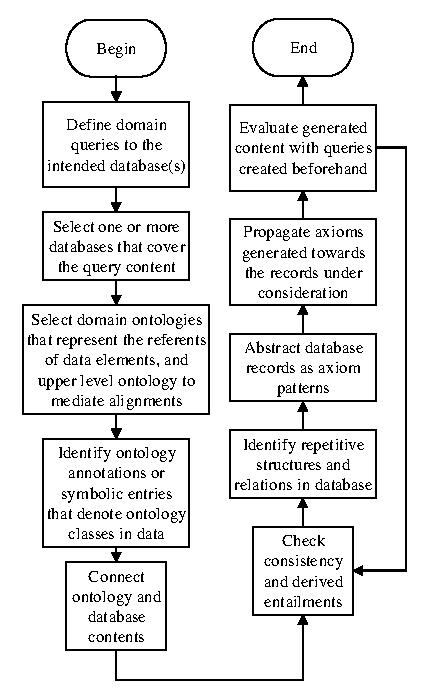
\includegraphics{./PIC/process}
	\caption{Ontology grounding process.}
	\label{fig:process}
\end{figure}


\begin{figure}[h!]
	\centering
	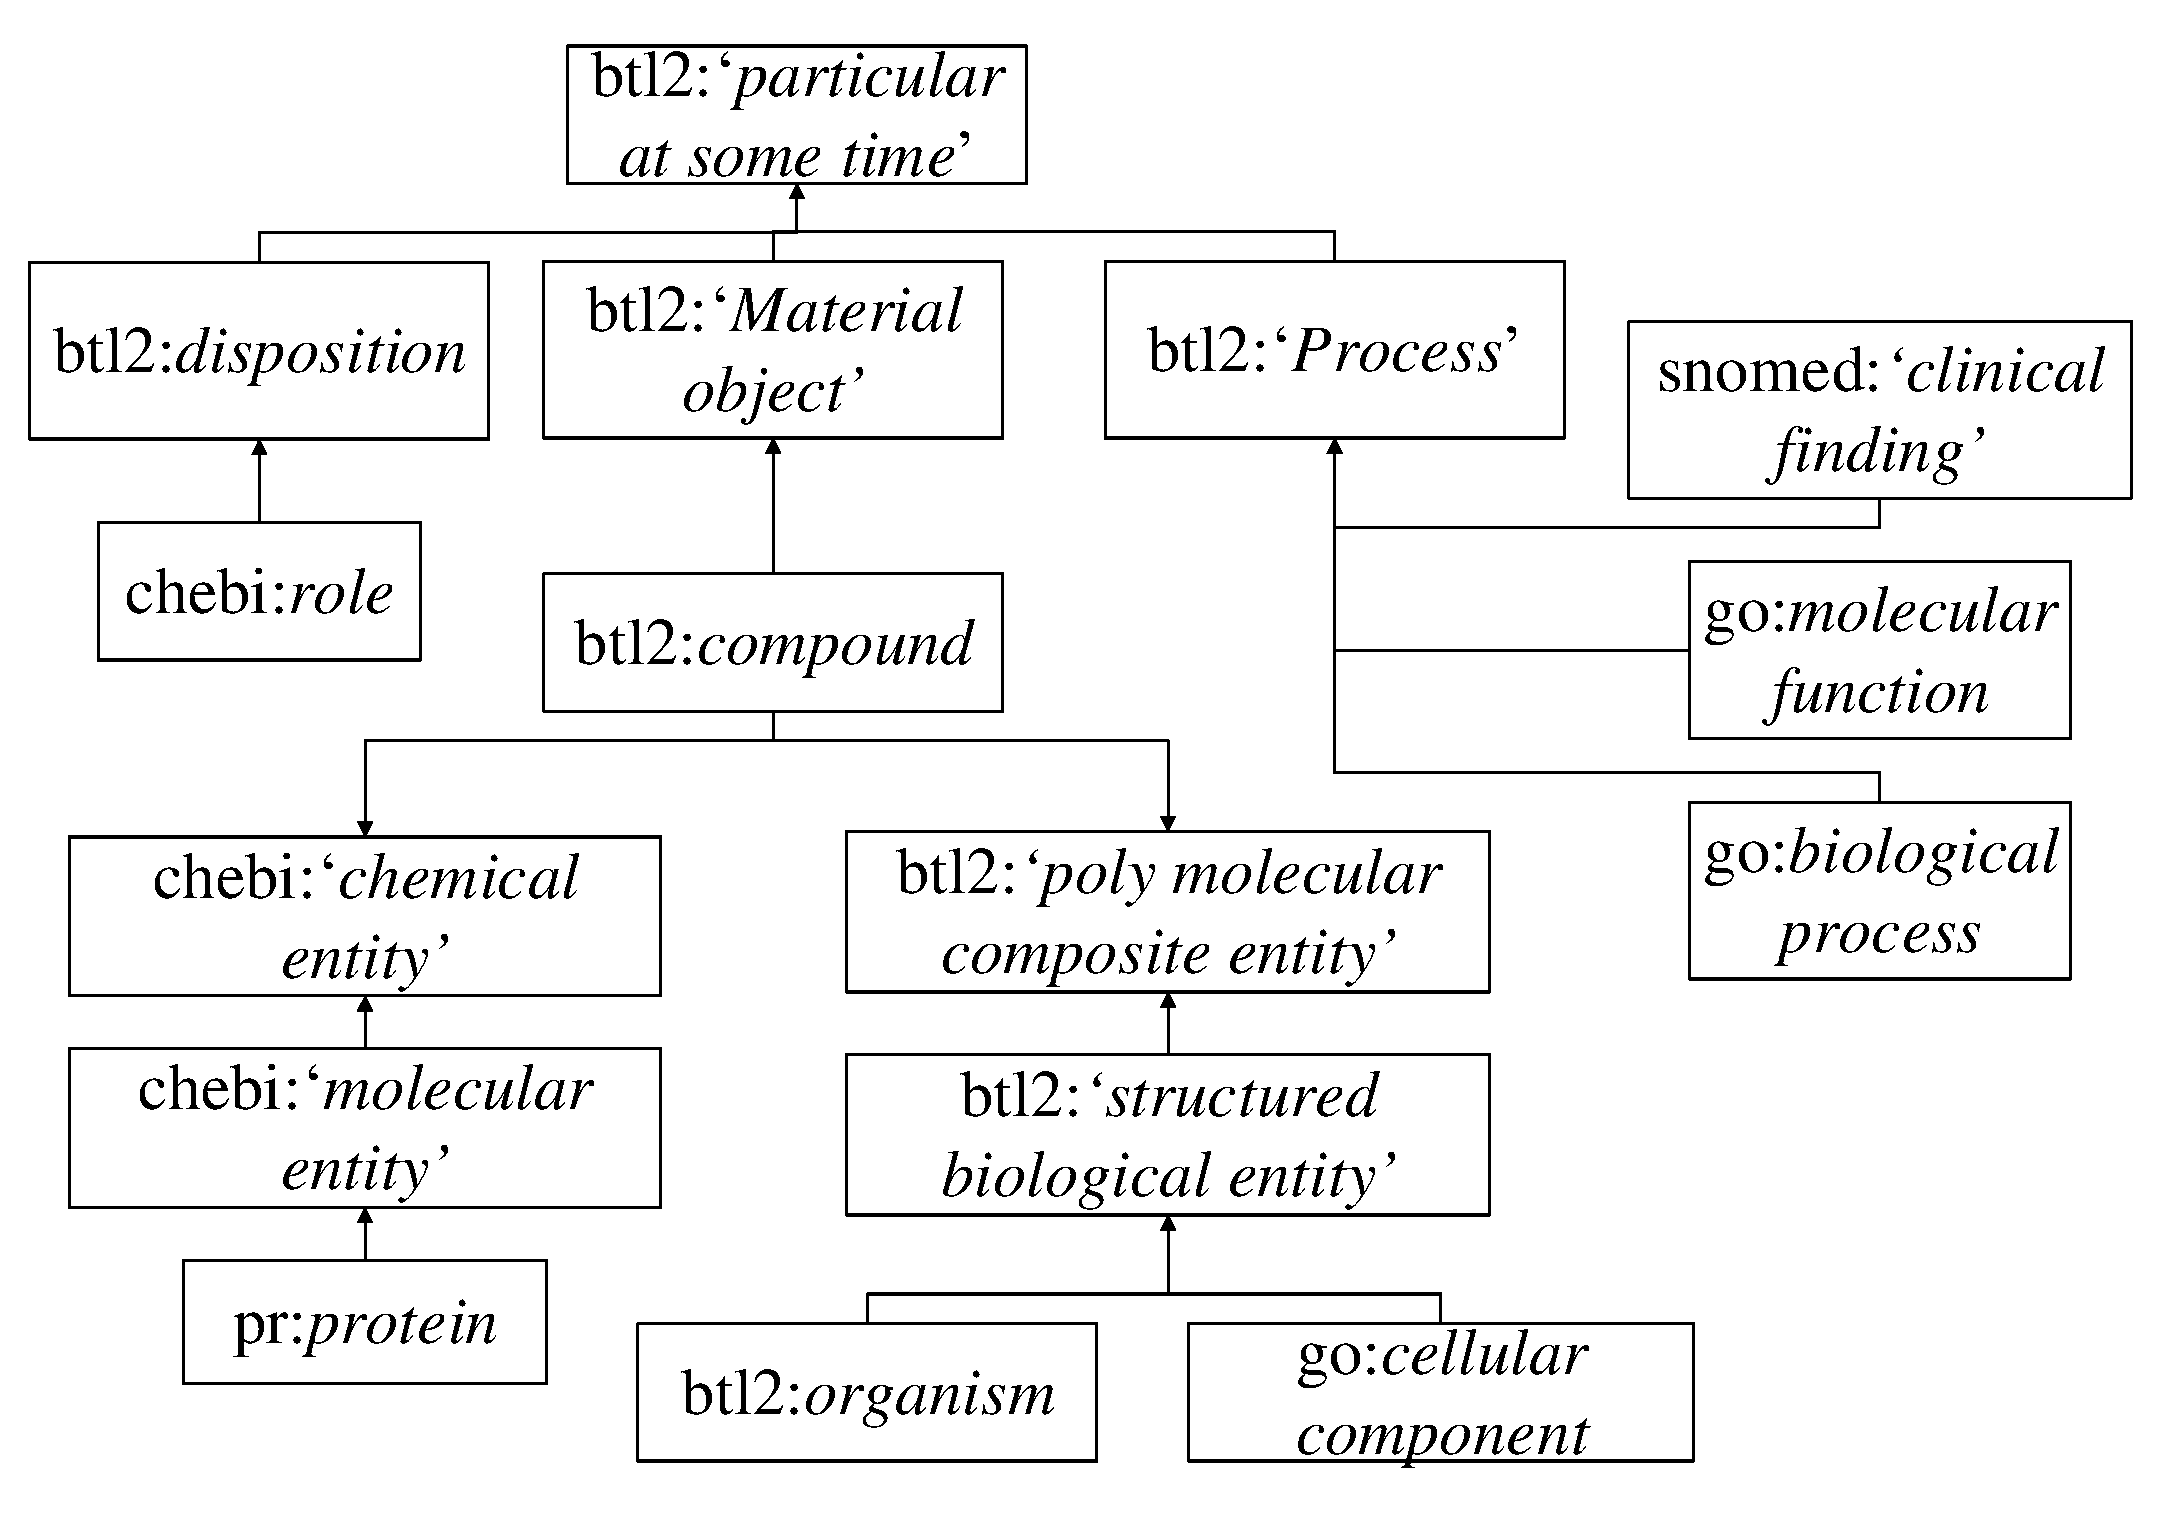
\includegraphics{/PIC/HierarquiaURI}
	\caption{Alignment of GO, ChEBI, SNOMED CT and PR under BTL2} 
	\label{fig:HierarquiaURI}
\end{figure}

%  \begin{figure}[h!]
%  \caption{\csentence{Sample figure title.}
%      A short description of the figure content
%      should go here.}
%      \end{figure}
%
%\begin{figure}[h!]
%  \caption{\csentence{Sample figure title.}
%      Figure legend text.}
%      \end{figure}

%%%%%%%%%%%%%%%%%%%%%%%%%%%%%%%%%%%
%%                               %%
%% Tables                        %%
%%                               %%
%%%%%%%%%%%%%%%%%%%%%%%%%%%%%%%%%%%

%% Use of \listoftables is discouraged.
%%
\section*{Tables}

\begin{table*}[h!]
	\begin{threeparttable}
		\caption{Uniprot and Ensembl table view}
		\label{table:uniprot}
		\centering
		\begin{tabular}{p{0.45in}p{0.4in}p{0.5in}p{0.8in}p{0.8in}p{0.6in}|p{1.25in}p{1.2in}} 
			\hline 
			Entry & Protein & Organism & GO (bp) & GO (mf) & GO (cc) & Ensembl ID & Ensembl Phenotype\\ \hline 
			F1MEW4 & CBS & \textit{Bos taurus} & blood vessel remodeling; \ldots & cystathionine $\beta$-synthase activity \ldots & cytoplasm \ldots & ENSBTAT00000000184; \ldots & No phenotype associated \\ 
			Q99707 & MS & \textit{Homo sapiens} & cobalamin metabolic process; \ldots & cobalamin binding; \ldots & cytoplasm \ldots & ENST00000366577; ENST00000535889 & Neural tube defect; Megaloblastic anemia; \ldots \\ \hline 
		\end{tabular}
		\begin{tablenotes}
			\item The left six columns contain UniProt entries; the two right columns correspond to Ensembl in entried. GO (bp) , GO (mf) and GO (cc) represents rows from UniProt that include annotations for GO classes '\textit{Biological process}', '\textit{Molecular function}' (understood as activity) and '\textit{Cellular component}'. IDs from UniProt and Ensembl are used for mapping purposes.\\ 
		\end{tablenotes}
	\end{threeparttable}
\end{table*}

\begin{table*}[h!]
	\centering
	\caption{Template table}
	\label{table:template}
	\begin{tabular}{p{0.3in}p{0.3in}p{0.3in}p{0.6in}p{0.6in}p{0.6in}p{0.6in}p{0.6in}} \hline 
		\# & \textit{P} &\textit{O} & \textit{Bp} & \textit{Mf} & \textit{C} & \textit{Ph} & \textit{M} \\ \hline 
		$k$ & $P_k$ & $O_k$ & $Bp_1\ldots n$ & $Mf_1\ldots n$ & $C_1\ldots n$ & $Ph1\ldots n$ & $M_1\ldots n$ \\
		\ldots & \ldots & \ldots & \ldots & \ldots & \ldots & \ldots & \ldots \\
		$l$ & $P_l$ & $O_l$ & $Bp_1\ldots n$ & $Mf_1\ldots n$ & $C_1\ldots n$ & $Ph1\ldots n$ & $M_1\ldots n$ \\
		\ldots & \ldots & \ldots & \ldots & \ldots & \ldots & \ldots & \ldots \\
		$m$ & $P_m$ & $O_m$ & $Bp_1\ldots n$ & $Mf_1\ldots n$ & $C_1\ldots n$ & $Ph1\ldots n$ & $M_1\ldots n$ \\ \hline 
	\end{tabular}
	\begin{tablenotes}
		\item The symbol \# represents record IDs; \textit{P} proteins; \textit{G} genes; \textit{O} organisms; \textit{Bp} biological processes;
		\textit{Mf} molecular function; \textit{C} cellular component; \textit{Ph} phenotype; and \textit{M} the associate molecules. \\ \\
	\end{tablenotes}
\end{table*}

\begin{table*}[h!]
	\begin{minipage}{\textwidth}
		\label{table:Summary}
		\caption{Survey of ontology sources, expressivity and reasoning performance in milliseconds}
		\centering
		\begin{tabular}{lrrrcrrrrrrrrr}
			\hline Ontology & Classes & Subcl. Axioms & Eq. Axioms & DL & Classification (h) & CQ1 & CQ2 & CQ3 & CQ4 & CQ5 & CQ6 \\ 
			x1  &  903 & 1,053  & 647 & $ALC$  & 586ms & 8ms & 13ms & 31ms & 35ms & 39ms  & 44ms \\ 
			x3 &  2,512 	& 2,957 & 1,945 & $ALC$  & 3,831ms & 12ms & 16ms & 32ms &  33ms & 38ms  &  39ms \\ 
			x10  & 8,599	 &  10,268 & 6,707 & $ALC$ & 38,994ms &70ms & 75ms & 85ms & 88ms & 92ms & 93ms \\ 
			%x30  & 25945 & 31072 & 20398 & $ALC$ & 397006ms  & 0ms & 1ms & 5ms  & 6ms  & ms &  ms  \\ 
			Modularized  & 2,838  & 4,071 & 1,203 & $SRI$ & 7,233,529ms & 373ms & 381ms & 385ms & 394ms & 397ms & 402ms \\ 
			\hline 
		\end{tabular} 
	\end{minipage}
\end{table*}
%\begin{table}[h!]
%\caption{Sample table title. This is where the description of the table should go.}
%      \begin{tabular}{cccc}
%        \hline
%           & B1  &B2   & B3\\ \hline
%        A1 & 0.1 & 0.2 & 0.3\\
%        A2 & ... & ..  & .\\
%        A3 & ..  & .   & .\\ \hline
%      \end{tabular}
%\end{table}

%%%%%%%%%%%%%%%%%%%%%%%%%%%%%%%%%%%
%%                               %%
%% Additional Files              %%
%%                               %%
%%%%%%%%%%%%%%%%%%%%%%%%%%%%%%%%%%%

%\section*{Additional Files}
%  \subsection*{Additional file 1 --- Sample additional file title}
%    Additional file descriptions text (including details of how to
%    view the file, if it is in a non-standard format or the file extension).  This might
%    refer to a multi-page table or a figure.
%
%  \subsection*{Additional file 2 --- Sample additional file title}
%    Additional file descriptions text.


\end{backmatter}
\end{document}
